% Формат А4, 14pt (ГОСТ Р 7.0.11-2011, 5.3.6)
\documentclass[a4paper,14pt]{extreport}

%%%%%%%%%%%%%%%%%%%%%%%%%%%%%%%%%%%%%%%%%%%%%%%%%%%%%%
%%%% Файл упрощённых настроек шаблона диссертации %%%%
%%%%%%%%%%%%%%%%%%%%%%%%%%%%%%%%%%%%%%%%%%%%%%%%%%%%%%

%%%        Подключение пакетов                 %%%
\usepackage{ifthen}                 % добавляет ifthenelse
%%% Инициализирование переменных, не трогать!  %%%
\newcounter{intvl}
\newcounter{otstup}
\newcounter{contnum}
\newcounter{pgnum}
\newcounter{bibliosel}
\newcounter{chapstyle}
\newcounter{headingdelim}
\newcounter{headingalign}
\newcounter{headingsize}
%%%%%%%%%%%%%%%%%%%%%%%%%%%%%%%%%%%%%%%%%%%%%%%%%%

%%% Область упрощённого управления оформлением %%%

%% Интервал между заголовками и между заголовком и текстом
% Заголовки отделяют от текста сверху и снизу тремя интервалами (ГОСТ Р 7.0.11-2011, 5.3.5)
\setcounter{intvl}{3}               % Коэффициент кратности к размеру шрифта

%% Отступы у заголовков в тексте
\setcounter{otstup}{0}              % 0 --- без отступа; 1 --- абзацный отступ

%% Нумерация формул, таблиц и рисунков
\setcounter{contnum}{0}             % 0 --- пораздельно (во введении подряд, без номера раздела); 1 --- сквозная нумерация по всей диссертации

%% Оглавление
\setcounter{pgnum}{1}               % 0 --- номера страниц никак не обозначены; 1 --- Стр. над номерами страниц (дважды компилировать после изменения)

%% Библиография
\setcounter{bibliosel}{0}           % 0 --- встроенная реализация с загрузкой файла через движок bibtex8; 1 --- реализация пакетом biblatex через движок biber

%% Текст и форматирование заголовков
\setcounter{chapstyle}{1}           % 0 --- разделы только под номером; 1 --- разделы с названием "Глава" перед номером
\setcounter{headingdelim}{1}        % 0 --- номер отделен пропуском в 1em или \quad; 1 --- номера разделов и приложений отделены точкой с пробелом, подразделы пропуском без точки; 2 --- номера разделов, подразделов и приложений отделены точкой с пробелом.

%% Выравнивание заголовков в тексте
\setcounter{headingalign}{0}        % 0 --- по центру; 1 --- по левому краю

%% Размеры заголовков в тексте
\setcounter{headingsize}{0}         % 0 --- по ГОСТ, все всегда 14 пт; 1 --- пропорционально изменяющийся размер в зависимости от базового шрифта
               % Упрощённые настройки шаблона 

%%% Проверка используемого TeX-движка %%%
\usepackage{iftex}
\newif\ifxetexorluatex   % определяем новый условный оператор (http://tex.stackexchange.com/a/47579/79756)
\ifXeTeX
    \xetexorluatextrue
\else
    \ifLuaTeX
        \xetexorluatextrue
    \else
        \xetexorluatexfalse
    \fi
\fi

%%% Поля и разметка страницы %%%
\usepackage{pdflscape}                              % Для включения альбомных страниц
\usepackage{geometry}                               % Для последующего задания полей

%%% Математические пакеты %%%
\usepackage{amsthm,amsfonts,amsmath,amssymb,amscd}  % Математические дополнения от AMS
\usepackage{mathtools}                              % Добавляет окружение multlined

%%%% Установки для размера шрифта 14 pt %%%%
%% Формирование переменных и констант для сравнения (один раз для всех подключаемых файлов)%%
%% должно располагаться до вызова пакета fontspec или polyglossia, потому что они сбивают его работу
\newlength{\curtextsize}
\newlength{\bigtextsize}
\setlength{\bigtextsize}{13.9pt}

\makeatletter
%\show\f@size                                       % неплохо для отслеживания, но вызывает стопорение процесса, если документ компилируется без команды  -interaction=nonstopmode 
\setlength{\curtextsize}{\f@size pt}
\makeatother

%%% Кодировки и шрифты %%%
\ifxetexorluatex
    \usepackage{polyglossia}                        % Поддержка многоязычности (fontspec подгружается автоматически)
\else
    \RequirePDFTeX                                  % tests for PDFTEX use and throws an error if a different engine is being used
    \usepackage{cmap}                               % Улучшенный поиск русских слов в полученном pdf-файле
    \usepackage[T2A]{fontenc}                       % Поддержка русских букв
    \usepackage[utf8]{inputenc}                     % Кодировка utf8
    \usepackage[english, russian]{babel}            % Языки: русский, английский
    \IfFileExists{pscyr.sty}{\usepackage{pscyr}}{}  % Красивые русские шрифты
\fi

%%% Оформление абзацев %%%
\usepackage{indentfirst}                            % Красная строка

%%% Цвета %%%
\usepackage[dvipsnames,usenames]{color}
\usepackage{colortbl}

%%% Таблицы %%%
\usepackage{longtable}                              % Длинные таблицы
\usepackage{multirow,makecell,array}                % Улучшенное форматирование таблиц
\usepackage{booktabs}                               % Возможность оформления таблиц в классическом книжном стиле (при правильном использовании не противоречит ГОСТ)
\usepackage[
singlelinecheck=false % <-- important
]{caption}

%%% Общее форматирование
\usepackage{soulutf8}                               % Поддержка переносоустойчивых подчёркиваний и зачёркиваний
\usepackage{icomma}                                 % Запятая в десятичных дробях


%%% Гиперссылки %%%
\usepackage{hyperref}

%%% Изображения %%%
\usepackage{graphicx}                               % Подключаем пакет работы с графикой

%%% Списки %%%
\usepackage{enumitem}

%%% Подписи %%%
\usepackage{caption}                                % Для управления подписями (рисунков и таблиц) % Может управлять номерами рисунков и таблиц с caption %Иногда может управлять заголовками в списках рисунков и таблиц
\usepackage{subcaption}                             % Работа с подрисунками и подобным

%%% Интервалы %%%
\usepackage[onehalfspacing]{setspace}               % Опция запуска пакета правит не только интервалы в обычном тексте, но и формульные

%%% Счётчики %%%
\usepackage[figure,table]{totalcount}               % Счётчик рисунков и таблиц
\usepackage{totcount}                               % Пакет создания счётчиков на основе последнего номера подсчитываемого элемента (может требовать дважды компилировать документ)
\usepackage{totpages}                               % Счётчик страниц, совместимый с hyperref (ссылается на номер последней страницы). Желательно ставить последним пакетом в преамбуле

  % Пакеты общие для диссертации и автореферата
%%% Колонтитулы %%%
\usepackage{fancyhdr}

%%% Прикладные пакеты %%% 
\usepackage{calc}               % Пакет для расчётов параметров, например длины
%\usepackage{etoolbox}          % ради функции patchcmd для управления списком литературы

\usepackage {interfaces-base}   % Набор базовых интерфейсов к некоторым пакетам, конкретные реализации загружаются в стиле

%%% Заголовки %%%
\usepackage{titlesec}           % Пакет настройки шрифтов заголовков в тексте

%%% Оглавление %%%
\usepackage{tocloft}

%%% Счётчики %%%
\usepackage{chngcntr}           % оперативная перенастройка счётчиков         % Пакеты для диссертации
\usepackage{tabularx,tabulary}  %таблицы с автоматически подбирающейся шириной столбцов


\usepackage{url}
\usepackage{hyperref}
\hypersetup{%
	colorlinks=true, 
	breaklinks=true, 
	urlcolor=blue, 
	linkcolor=blue, 
	citecolor=blue, 
} %%%

\usepackage{graphicx}
\usepackage{wrapfig}
\usepackage{lipsum}  % generates filler text

% Листинги с исходным кодом программ
\usepackage{fancyvrb}
\usepackage{listings}

% Плавающие окружения. во многом лучше пакета float
\usepackage{floatrow}
%Диаграммы Фейнмана
\usepackage{tikz}
\usetikzlibrary{trees}
\usetikzlibrary{decorations.pathmorphing}
\usetikzlibrary{decorations.markings}
\usetikzlibrary{positioning, automata, arrows, arrows.meta}

\usepackage{longtable} %Длинные таблицы
\usepackage{pdfpages}   %Вставлять пдф
\usepackage{afterpage} %Пустая страница
\usepackage{anyfontsize}

\usepackage{titlesec}
\usepackage{physics}
\DeclareMathOperator{\sinc}{sinc}

\pagestyle{fancy}
\fancyhf{}
%\fancyhead[LE,RO]{Share\LaTeX}
%\fancyhead[RE,LO]{Guides and tutorials}
%\fancyfoot[CE,CO]{\leftmark}
\fancyfoot[LE,RO]{\thepage}
\renewcommand{\headrulewidth}{0pt}

\usepackage{datatool}
%\usepackage{siunitx}
\usepackage{booktabs} % for nicer tables
%\usepackage{caption} % improve caption spacing (among other things)
\usepackage{bm}
\renewcommand*\dtldisplaystarttab{\toprule}
\renewcommand*\dtldisplayendtab{\tabularnewline\bottomrule}
\renewcommand*\dtldisplayafterhead{\midrule}

\usepackage{pgfplotstable}
\usepackage{siunitx}
\usepackage{booktabs}

\usepackage{hyperref}

\usepackage{fancyhdr}

        % Пакеты для специфических пользовательских задач
%%% Переопределение именований, чтобы можно было и в преамбуле использовать %%%
\renewcommand{\chaptername}{Глава}
\renewcommand{\appendixname}{Приложение} % (ГОСТ Р 7.0.11-2011, 5.7)
\newcommand\DoubleLine[5][3pt]{%
  \path(#2)--(#3)coordinate[at start](h1)coordinate[at end](h2);
  \draw[#4]($(h1)!#1!90:(h2)$)--($(h2)!#1!-90:(h1)$);
  \draw[#5]($(h1)!#1!-90:(h2)$)--($(h2)!#1!90:(h1)$);
}       % Переопределение именований, чтобы можно было и в преамбуле использовать
%%% Макет страницы %%%
% Выставляем значения полей (ГОСТ 7.0.11-2011, 5.3.7)
\geometry{a4paper,top=2cm,bottom=2cm,left=3cm,right=2cm}

%%% Кодировки и шрифты %%%
\ifxetexorluatex
    \setmainlanguage[babelshorthands=true]{russian}  % Язык по-умолчанию русский с поддержкой приятных команд пакета babel
    \setotherlanguage{english}                       % Дополнительный язык = английский (в американской вариации по-умолчанию)
    \ifXeTeX
        \defaultfontfeatures{Ligatures=TeX,Mapping=tex-text}
    \else
        \defaultfontfeatures{Ligatures=TeX}
    \fi
    \setmainfont{Times New Roman}
    \newfontfamily\cyrillicfont{Times New Roman}
    \setsansfont{Arial}
    \newfontfamily\cyrillicfontsf{Arial}
    \setmonofont{Courier New}
    \newfontfamily\cyrillicfonttt{Courier New}
\else
    \IfFileExists{pscyr.sty}{\renewcommand{\rmdefault}{ftm}}{}
\fi

%%% Интервалы %%%
%linespread-реализация ближе к реализации полуторного интервала в ворде.
%setspace реализация заточена под шрифты 10, 11, 12pt, под остальные кегли хуже, но всё же ближе к типографской классике. 
%\linespread{1.3}                    % Полуторный интервал (ГОСТ Р 7.0.11-2011, 5.3.6)

%%% Выравнивание и переносы %%%
\sloppy                             % Избавляемся от переполнений
\clubpenalty=10000                  % Запрещаем разрыв страницы после первой строки абзаца
\widowpenalty=10000                 % Запрещаем разрыв страницы после последней строки абзаца

%%% Изображения %%%
\graphicspath{{images/}}            % Пути к изображениям

%%% Подписи %%%
\captionsetup{%
singlelinecheck=off,                % Многострочные подписи, например у таблиц
skip=2pt,                           % Вертикальная отбивка между подписью и содержимым рисунка или таблицы определяется ключом
justification=centering,            % Центрирование подписей, заданных командой \caption
}

%%% Рисунки %%%
\DeclareCaptionLabelSeparator*{emdash}{~--- }             % (ГОСТ 2.105, 4.3.1)
\captionsetup[figure]{labelsep=emdash,font=onehalfspacing,position=bottom}

%%% Таблицы %%%
\DeclareCaptionFormat{tablecaption}{\raggedleft #1#2\\%   % Идентификатор таблицы справа, на отдельной строке
    \centering{#3}}                                       % Наименование таблицы строкой ниже и центрировано, без переносов
\DeclareCaptionFormat{tablenocaption}{\raggedleft #1#2%   % Идентификатор таблицы справа, на отдельной строке
}                                                         % Наименование таблицы отсутствует
\captionsetup[table]{format=tablecaption,labelsep=space,singlelinecheck=off,font=onehalfspacing,position=top}  % пробельный разделитель идентификатора с номером от наименования, многострочные наименования и прочее
\DeclareCaptionLabelFormat{continued}{Продолжение таблицы~#2}

%%% Подписи подрисунков %%%
\renewcommand{\thesubfigure}{\asbuk{subfigure}}           % Буквенные номера подрисунков
\captionsetup[subfigure]{font={normalsize},               % Шрифт подписи названий подрисунков (не отличается от основного)
    labelformat=brace,                                    % Формат обозначения подрисунка
    justification=centering,                              % Выключка подписей (форматирование), один из вариантов            
}
%\DeclareCaptionFont{font12pt}{\fontsize{12pt}{13pt}\selectfont} % объявляем шрифт 12pt для использования в подписях, тут же надо интерлиньяж объявлять, если не наследуется
%\captionsetup[subfigure]{font={font12pt}}                 % Шрифт подписи названий подрисунков (всегда 12pt)

%%% Цвета гиперссылок %%%
\definecolor{linkcolor}{rgb}{0,0,0}
\definecolor{citecolor}{rgb}{0,0,0}
\definecolor{urlcolor}{rgb}{0,0,0}

%%% Настройки гиперссылок %%%
\hypersetup{
    linktocpage=true,           % ссылки с номера страницы в оглавлении, списке таблиц и списке рисунков
%    pdfpagelabels=false,        % set PDF page labels (true|false)
    plainpages=false,           % Forces page anchors to be named by the Arabic form  of the page number, rather than the formatted form
    colorlinks,                 % ссылки отображаются раскрашенным текстом, а не раскрашенным прямоугольником, вокруг текста
    linkcolor={linkcolor},      % цвет ссылок типа ref, eqref и подобных
    citecolor={citecolor},      % цвет ссылок-цитат
    urlcolor={urlcolor},        % цвет гиперссылок
}

\ifLuaTeX
    \hypersetup{
        unicode,                % Unicode encoded PDF strings
    }
\fi

%%% Шаблон %%%
\DeclareRobustCommand{\todo}{\textcolor{black}}       % решаем проблему превращения названия цвета в результате \MakeUppercase, http://tex.stackexchange.com/a/187930/79756 , \DeclareRobustCommand protects \todo from expanding inside \MakeUppercase
\setlength{\parindent}{2.5em}                       % Абзацный отступ. Должен быть одинаковым по всему тексту и равен пяти знакам (ГОСТ Р 7.0.11-2011, 5.3.7).

%%% Списки %%%
% Используем дефис для ненумерованных списков (ГОСТ 2.105-95, 4.1.7)
\renewcommand{\labelitemi}{\normalfont\bfseries{--}} 
\setlist{nosep,%                                    % Единый стиль для всех списков (пакет enumitem), без дополнительных интервалов.
    labelindent=\parindent,leftmargin=*%            % Каждый пункт, подпункт и перечисление записывают с абзацного отступа (ГОСТ 2.105-95, 4.1.8)
}
    % Стили общие для диссертации и автореферата
\LoadInterface {titlesec}                   % Подгружаем интерфейсы для дополнительных опций управления некоторыми пакетами

%%% Блок управления параметрами для выравнивания заголовков в тексте %%%
\newlength{\otstuplen}
\setlength{\otstuplen}{\theotstup\parindent}
\ifthenelse{\equal{\theheadingalign}{0}}{% выравнивание заголовков в тексте
    \newcommand{\hdngalign}{\filcenter}                % по центру
    \newcommand{\hdngaligni}{\hfill\hspace{\otstuplen}}% по центру
}{%
    \newcommand{\hdngalign}{\filright}                 % по левому краю
    \newcommand{\hdngaligni}{\hspace{\otstuplen}}      % по левому краю
} % В обоих случаях вроде бы без переноса, как и надо (ГОСТ Р 7.0.11-2011, 5.3.5)

%%% Оглавление %%%
\renewcommand{\cftchapdotsep}{\cftdotsep}                % отбивка точками до номера страницы начала главы/раздела
\renewcommand{\cfttoctitlefont}{\hdngaligni\fontsize{14pt}{16pt}\selectfont\bfseries}% вместе со следующей строкой
\renewcommand{\cftaftertoctitle}{\hfill}                 % устанавливает заголовок по центру
\setlength{\cftbeforetoctitleskip}{-1.4\curtextsize}     % Поскольку этот заголовок всегда является первым на странице, то перед ним отделять пустым тройным интервалом не следует. Независимо от основного шрифта, в этом случае зануление (почти) происходит при -1.4\curtextsize.
\setlength{\cftaftertoctitleskip}{\theintvl\curtextsize} % Если считаем Оглавление заголовком, то выставляем после него тройной интервал через наше определённое значение

%% Переносить слова в заголовке не допускается (ГОСТ Р 7.0.11-2011, 5.3.5). Заголовки в оглавлении должны точно повторять заголовки в тексте (ГОСТ Р 7.0.11-2011, 5.2.3). Прямого указания на запрет переносов в оглавлении нет, но по той же логике невнесения искажений в смысл, лучше в оглавлении не переносить:
\cftsetrmarg{2.55em plus1fil}                       %To have the (sectional) titles in the ToC, etc., typeset ragged right with no hyphenation
\renewcommand{\cftchappagefont}{\normalfont}        % нежирные номера страниц у глав в оглавлении
\renewcommand{\cftchapleader}{\cftdotfill{\cftchapdotsep}}% нежирные точки до номеров страниц у глав в оглавлении
%\renewcommand{\cftchapfont}{}                       % нежирные названия глав в оглавлении

\ifthenelse{\theheadingdelim > 0}{%
    \renewcommand\cftchapaftersnum{.\ }   % добавляет точку с пробелом после номера раздела в оглавлении
}{%
\renewcommand\cftchapaftersnum{\quad}     % добавляет \quad после номера раздела в оглавлении
}
\ifthenelse{\theheadingdelim > 1}{%
    \renewcommand\cftsecaftersnum{.\ }    % добавляет точку с пробелом после номера подраздела в оглавлении
    \renewcommand\cftsubsecaftersnum{.\ } % добавляет точку с пробелом после номера подподраздела в оглавлении
}{%
\renewcommand\cftsecaftersnum{\quad}      % добавляет \quad после номера подраздела в оглавлении
\renewcommand\cftsubsecaftersnum{\quad}   % добавляет \quad после номера подподраздела в оглавлении
}

\ifthenelse{\equal{\thepgnum}{1}}{%
    \addtocontents{toc}{~\hfill{Стр.}\par}% добавить Стр. над номерами страниц
}

%%% Оформление названий глав %%%
%% настройки заголовка списка рисунков
\renewcommand{\cftloftitlefont}{\hdngaligni\fontsize{14pt}{16pt}\selectfont\bfseries}% вместе со следующей строкой
\renewcommand{\cftafterloftitle}{\hfill}                                             % устанавливает заголовок по центру
\setlength{\cftbeforeloftitleskip}{-1.5\curtextsize}     % Поскольку этот заголовок всегда является первым на странице, то перед ним отделять пустым тройным интервалом не следует. Независимо от основного шрифта, в этом случае зануление (почти) происходит при -1.5\curtextsize.
\setlength{\cftafterloftitleskip}{\theintvl\curtextsize} % выставляем после него тройной интервал через наше определённое значение

%% настройки заголовка списка таблиц
\renewcommand{\cftlottitlefont}{\hdngaligni\fontsize{14pt}{16pt}\selectfont\bfseries}% вместе со следующей строкой
\renewcommand{\cftafterlottitle}{\hfill}                                             % устанавливает заголовок по центру
\setlength{\cftbeforelottitleskip}{-1.5\curtextsize}     % Поскольку этот заголовок всегда является первым на странице, то перед ним отделять пустым тройным интервалом не следует. Независимо от основного шрифта, в этом случае зануление (почти) происходит при -1.5\curtextsize.
\setlength{\cftafterlottitleskip}{\theintvl\curtextsize} % выставляем после него тройной интервал через наше определённое значение

\ifnum\curtextsize>\bigtextsize     % Проверяем условие использования базового шрифта 14 pt
\setlength{\headheight}{17pt}       % Исправляем высоту заголовка
\else
\setlength{\headheight}{15pt}       % Исправляем высоту заголовка
\fi

%%% Колонтитулы %%%
% Порядковый номер страницы печатают на середине верхнего поля страницы (ГОСТ Р 7.0.11-2011, 5.3.8)
\makeatletter
\let\ps@plain\ps@fancy              % Подчиняем первые страницы каждой главы общим правилам
\makeatother
\pagestyle{fancy}                   % Меняем стиль оформления страниц
\fancyhf{}                          % Очищаем текущие значения
\fancyfoot[C]{\thepage}             % Печатаем номер страницы на середине верхнего поля
\renewcommand{\headrulewidth}{0pt}  % Убираем разделительную линию

%%% Оформление заголовков глав, разделов, подразделов %%%
%% Работа должна быть выполнена ... размером шрифта 12-14 пунктов (ГОСТ Р 7.0.11-2011, 5.3.8). То есть не должно быть надписей шрифтом более 14. Так и поставим.
%% Эти установки будут давать одинаковый результат независимо от выбора базовым шрифтом 12 пт или 14 пт
\titleformat{\chapter}[block]                                % default display;  hang = with a hanging label. (Like the standard \section.); block = typesets the whole title in a block (a paragraph) without additional formatting. Useful in centered titles
        {\hdngalign\fontsize{14pt}{16pt}\selectfont\bfseries}% 
        %\fontsize{<size>}{<skip>} % второе число ставим 1.2*первое, чтобы адекватно отрабатывали команды по расчету полуторного интервала (домножая разные комбинации коэффициентов на этот)
        {\thechapter\cftchapaftersnum}                       % Заголовки в оглавлении должны точно повторять заголовки в тексте (ГОСТ Р 7.0.11-2011, 5.2.3).
        {0em}% отступ от номера до текста
        {}%

\titleformat{\section}[block]                                % default hang;  hang = with a hanging label. (Like the standard \section.); block = typesets the whole title in a block (a paragraph) without additional formatting. Useful in centered titles
        {\hdngalign\fontsize{14pt}{16pt}\selectfont\bfseries}% 
        %\fontsize{<size>}{<skip>} % второе число ставим 1.2*первое, чтобы адекватно отрабатывали команды по расчету полуторного интервала (домножая разные комбинации коэффициентов на этот)
        {\thesection\cftsecaftersnum}                        % Заголовки в оглавлении должны точно повторять заголовки в тексте (ГОСТ Р 7.0.11-2011, 5.2.3).
        {0em}% отступ от номера до текста
        {}%

\titleformat{\subsection}[block]                             % default hang;  hang = with a hanging label. (Like the standard \section.); block = typesets the whole title in a block (a paragraph) without additional formatting. Useful in centered titles
        {\hdngalign\fontsize{14pt}{16pt}\selectfont\bfseries}% 
        %\fontsize{<size>}{<skip>} % второе число ставим 1.2*первое, чтобы адекватно отрабатывали команды по расчету полуторного интервала (домножая разные комбинации коэффициентов на этот)
        {\thesubsection\cftsubsecaftersnum}                  % Заголовки в оглавлении должны точно повторять заголовки в тексте (ГОСТ Р 7.0.11-2011, 5.2.3).
        {0em}% отступ от номера до текста
        {}%

\ifthenelse{\equal{\thechapstyle}{1}}{%
    \sectionformat{\chapter}{% Параметры заголовков разделов в тексте
        label=\chaptername\ \thechapter\cftchapaftersnum,
        labelsep=0em,
    }
    %% Следующие две строки: будет вписано слово Глава перед каждым номером раздела в оглавлении   
    \renewcommand{\cftchappresnum}{\chaptername\ }
    \setlength{\cftchapnumwidth}{\widthof{\cftchapfont\cftchappresnum\thechapter\cftchapaftersnum}}
}%

%% Интервалы между заголовками
% На эти величины titlespacing множит через *
\beforetitleunit=\curtextsize% привязались к нашему размеру шрифта
\aftertitleunit=\curtextsize% привязались к нашему размеру шрифта

% Счётчик intvl и длина \otstup определены в файле setup
\titlespacing{\chapter}{\theotstup\parindent}{-1.7em}{*\theintvl}       % Заголовки отделяют от текста сверху и снизу тремя интервалами (ГОСТ Р 7.0.11-2011, 5.3.5). Поскольку название главы всегда является первым на странице, то перед ним отделять пустым тройным интервалом не следует. Независимо от основного шрифта, в этом случае зануление происходит при -1.7em.
\titlespacing{\section}{\theotstup\parindent}{*\theintvl}{*\theintvl}
\titlespacing{\subsection}{\theotstup\parindent}{*\theintvl}{*\theintvl}
\titlespacing{\subsubsection}{\theotstup\parindent}{*\theintvl}{*\theintvl}

%%% Блок дополнительного управления размерами заголовков
\ifthenelse{\equal{\theheadingsize}{1}}{% Пропорциональные заголовки и базовый шрифт 14 пт
    \renewcommand{\cfttoctitlefont}{\hdngaligni\Large\bfseries} % Исправляем размер заголовка оглавления
    \setlength{\cftbeforetoctitleskip}{-1.2\curtextsize}        % Исправляем вертикальный отступ перед заголовком оглавления
    \renewcommand{\cftloftitlefont}{\hdngaligni\Large\bfseries} % Исправляем размер заголовка списка рисунков
    \setlength{\cftbeforeloftitleskip}{-1.4\curtextsize}        % Исправляем вертикальный отступ перед заголовком списка рисунков
    \renewcommand{\cftlottitlefont}{\hdngaligni\Large\bfseries} % Исправляем размер заголовка списка таблиц 
    \setlength{\cftbeforelottitleskip}{-1.4\curtextsize}        % Исправляем вертикальный отступ перед заголовком списка таблиц
    \sectionformat{\chapter}{% Параметры заголовков разделов в тексте
        format=\hdngalign\Large\bfseries, % Исправляем размер заголовка
        top-=0.4em,                       % Исправляем вертикальный отступ перед заголовком
    }
    \sectionformat{\section}{% Параметры заголовков подразделов в тексте
        format=\hdngalign\large\bfseries, % Исправляем размер заголовка
    }
}

\ifthenelse{\equal{\theheadingsize}{1}\AND \curtextsize < \bigtextsize}{% Пропорциональные заголовки и базовый шрифт 14 пт
    \sectionformat{\chapter}{% Параметры заголовков разделов в тексте
        top-=0.2em, % Исправляем вертикальный отступ перед заголовком
    }
}

%%% Счётчики %%%

%% Упрощённые настройки шаблона диссертации: нумерация формул, таблиц, рисунков
\ifthenelse{\equal{\thecontnum}{1}}{%
    \counterwithout{equation}{chapter} % Убираем связанность номера формулы с номером главы/раздела
    \counterwithout{figure}{chapter}   % Убираем связанность номера рисунка с номером главы/раздела
    \counterwithout{table}{chapter}    % Убираем связанность номера таблицы с номером главы/раздела
}

%%http://www.linux.org.ru/forum/general/6993203#comment-6994589 (используется totcount)
\makeatletter
\def\formbytotal#1#2#3#4#5{%
    \newcount\@c
    \@c\totvalue{#1}\relax
    \newcount\@last
    \newcount\@pnul
    \@last\@c\relax
    \divide\@last 10
    \@pnul\@last\relax
    \divide\@pnul 10
    \multiply\@pnul-10
    \advance\@pnul\@last
    \multiply\@last-10
    \advance\@last\@c
    \total{#1}~#2%
    \ifnum\@pnul=1#5\else%
    \ifcase\@last#5\or#3\or#4\or#4\or#4\else#5\fi
    \fi
}
\makeatother
           % Стили для диссертации
% для вертикального центрирования ячеек в tabulary
\def\zz{\ifx\[$\else\aftergroup\zzz\fi}
\def\zzz{\setbox0\lastbox
\dimen0\dimexpr\extrarowheight + \ht0-\dp0\relax
\setbox0\hbox{\raise-.5\dimen0\box0}%
\ht0=\dimexpr\ht0+\extrarowheight\relax
\dp0=\dimexpr\dp0+\extrarowheight\relax 
\box0
}



\lstdefinelanguage{Renhanced}%
{keywords={abbreviate,abline,abs,acos,acosh,action,add1,add,%
        aggregate,alias,Alias,alist,all,anova,any,aov,aperm,append,apply,%
        approx,approxfun,apropos,Arg,args,array,arrows,as,asin,asinh,%
        atan,atan2,atanh,attach,attr,attributes,autoload,autoloader,ave,%
        axis,backsolve,barplot,basename,besselI,besselJ,besselK,besselY,%
        beta,binomial,body,box,boxplot,break,browser,bug,builtins,bxp,by,%
        c,C,call,Call,case,cat,category,cbind,ceiling,character,char,%
        charmatch,check,chol,chol2inv,choose,chull,class,close,cm,codes,%
        coef,coefficients,co,col,colnames,colors,colours,commandArgs,%
        comment,complete,complex,conflicts,Conj,contents,contour,%
        contrasts,contr,control,helmert,contrib,convolve,cooks,coords,%
        distance,coplot,cor,cos,cosh,count,fields,cov,covratio,wt,CRAN,%
        create,crossprod,cummax,cummin,cumprod,cumsum,curve,cut,cycle,D,%
        data,dataentry,date,dbeta,dbinom,dcauchy,dchisq,de,debug,%
        debugger,Defunct,default,delay,delete,deltat,demo,de,density,%
        deparse,dependencies,Deprecated,deriv,description,detach,%
        dev2bitmap,dev,cur,deviance,off,prev,,dexp,df,dfbetas,dffits,%
        dgamma,dgeom,dget,dhyper,diag,diff,digamma,dim,dimnames,dir,%
        dirname,dlnorm,dlogis,dnbinom,dnchisq,dnorm,do,dotplot,double,%
        download,dpois,dput,drop,drop1,dsignrank,dt,dummy,dump,dunif,%
        duplicated,dweibull,dwilcox,dyn,edit,eff,effects,eigen,else,%
        emacs,end,environment,env,erase,eval,equal,evalq,example,exists,%
        exit,exp,expand,expression,External,extract,extractAIC,factor,%
        fail,family,fft,file,filled,find,fitted,fivenum,fix,floor,for,%
        For,formals,format,formatC,formula,Fortran,forwardsolve,frame,%
        frequency,ftable,ftable2table,function,gamma,Gamma,gammaCody,%
        gaussian,gc,gcinfo,gctorture,get,getenv,geterrmessage,getOption,%
        getwd,gl,glm,globalenv,gnome,GNOME,graphics,gray,grep,grey,grid,%
        gsub,hasTsp,hat,heat,help,hist,home,hsv,httpclient,I,identify,if,%
        ifelse,Im,image,\%in\%,index,influence,measures,inherits,install,%
        installed,integer,interaction,interactive,Internal,intersect,%
        inverse,invisible,IQR,is,jitter,kappa,kronecker,labels,lapply,%
        layout,lbeta,lchoose,lcm,legend,length,levels,lgamma,library,%
        licence,license,lines,list,lm,load,local,locator,log,log10,log1p,%
        log2,logical,loglin,lower,lowess,ls,lsfit,lsf,ls,machine,Machine,%
        mad,mahalanobis,make,link,margin,match,Math,matlines,mat,matplot,%
        matpoints,matrix,max,mean,median,memory,menu,merge,methods,min,%
        missing,Mod,mode,model,response,mosaicplot,mtext,mvfft,na,nan,%
        names,omit,nargs,nchar,ncol,NCOL,new,next,NextMethod,nextn,%
        nlevels,nlm,noquote,NotYetImplemented,NotYetUsed,nrow,NROW,null,%
        numeric,\%o\%,objects,offset,old,on,Ops,optim,optimise,optimize,%
        options,or,order,ordered,outer,package,packages,page,pairlist,%
        pairs,palette,panel,par,parent,parse,paste,path,pbeta,pbinom,%
        pcauchy,pchisq,pentagamma,persp,pexp,pf,pgamma,pgeom,phyper,pico,%
        pictex,piechart,Platform,plnorm,plogis,plot,pmatch,pmax,pmin,%
        pnbinom,pnchisq,pnorm,points,poisson,poly,polygon,polyroot,pos,%
        postscript,power,ppoints,ppois,predict,preplot,pretty,Primitive,%
        print,prmatrix,proc,prod,profile,proj,prompt,prop,provide,%
        psignrank,ps,pt,ptukey,punif,pweibull,pwilcox,q,qbeta,qbinom,%
        qcauchy,qchisq,qexp,qf,qgamma,qgeom,qhyper,qlnorm,qlogis,qnbinom,%
        qnchisq,qnorm,qpois,qqline,qqnorm,qqplot,qr,Q,qty,qy,qsignrank,%
        qt,qtukey,quantile,quasi,quit,qunif,quote,qweibull,qwilcox,%
        rainbow,range,rank,rbeta,rbind,rbinom,rcauchy,rchisq,Re,read,csv,%
        csv2,fwf,readline,socket,real,Recall,rect,reformulate,regexpr,%
        relevel,remove,rep,repeat,replace,replications,report,require,%
        resid,residuals,restart,return,rev,rexp,rf,rgamma,rgb,rgeom,R,%
        rhyper,rle,rlnorm,rlogis,rm,rnbinom,RNGkind,rnorm,round,row,%
        rownames,rowsum,rpois,rsignrank,rstandard,rstudent,rt,rug,runif,%
        rweibull,rwilcox,sample,sapply,save,scale,scan,scan,screen,sd,se,%
        search,searchpaths,segments,seq,sequence,setdiff,setequal,set,%
        setwd,show,sign,signif,sin,single,sinh,sink,solve,sort,source,%
        spline,splinefun,split,sqrt,stars,start,stat,stem,step,stop,%
        storage,strstrheight,stripplot,strsplit,structure,strwidth,sub,%
        subset,substitute,substr,substring,sum,summary,sunflowerplot,svd,%
        sweep,switch,symbol,symbols,symnum,sys,status,system,t,table,%
        tabulate,tan,tanh,tapply,tempfile,terms,terrain,tetragamma,text,%
        time,title,topo,trace,traceback,transform,tri,trigamma,trunc,try,%
        ts,tsp,typeof,unclass,undebug,undoc,union,unique,uniroot,unix,%
        unlink,unlist,unname,untrace,update,upper,url,UseMethod,var,%
        variable,vector,Version,vi,warning,warnings,weighted,weights,%
        which,while,window,write,\%x\%,x11,X11,xedit,xemacs,xinch,xor,%
        xpdrows,xy,xyinch,yinch,zapsmall,zip},%
    otherkeywords={!,!=,~,$,*,\%,\&,\%/\%,\%*\%,\%\%,<-,<<-},%
    alsoother={._$},%
    sensitive,%
    morecomment=[l]\#,%
    morestring=[d]",%
    morestring=[d]'% 2001 Robert Denham
}%

%решаем проблему с кириллицей в комментариях (в pdflatex) https://tex.stackexchange.com/a/103712/79756
\lstset{extendedchars=true,literate={Ö}{{\"O}}1
    {Ä}{{\"A}}1
    {Ü}{{\"U}}1
    {ß}{{\ss}}1
    {ü}{{\"u}}1
    {ä}{{\"a}}1
    {ö}{{\"o}}1
    {~}{{\textasciitilde}}1
    {а}{{\selectfont\char224}}1
    {б}{{\selectfont\char225}}1
    {в}{{\selectfont\char226}}1
    {г}{{\selectfont\char227}}1
    {д}{{\selectfont\char228}}1
    {е}{{\selectfont\char229}}1
    {ё}{{\"e}}1
    {ж}{{\selectfont\char230}}1
    {з}{{\selectfont\char231}}1
    {и}{{\selectfont\char232}}1
    {й}{{\selectfont\char233}}1
    {к}{{\selectfont\char234}}1
    {л}{{\selectfont\char235}}1
    {м}{{\selectfont\char236}}1
    {н}{{\selectfont\char237}}1
    {о}{{\selectfont\char238}}1
    {п}{{\selectfont\char239}}1
    {р}{{\selectfont\char240}}1
    {с}{{\selectfont\char241}}1
    {т}{{\selectfont\char242}}1
    {у}{{\selectfont\char243}}1
    {ф}{{\selectfont\char244}}1
    {х}{{\selectfont\char245}}1
    {ц}{{\selectfont\char246}}1
    {ч}{{\selectfont\char247}}1
    {ш}{{\selectfont\char248}}1
    {щ}{{\selectfont\char249}}1
    {ъ}{{\selectfont\char250}}1
    {ы}{{\selectfont\char251}}1
    {ь}{{\selectfont\char252}}1
    {э}{{\selectfont\char253}}1
    {ю}{{\selectfont\char254}}1
    {я}{{\selectfont\char255}}1
    {А}{{\selectfont\char192}}1
    {Б}{{\selectfont\char193}}1
    {В}{{\selectfont\char194}}1
    {Г}{{\selectfont\char195}}1
    {Д}{{\selectfont\char196}}1
    {Е}{{\selectfont\char197}}1
    {Ё}{{\"E}}1
    {Ж}{{\selectfont\char198}}1
    {З}{{\selectfont\char199}}1
    {И}{{\selectfont\char200}}1
    {Й}{{\selectfont\char201}}1
    {К}{{\selectfont\char202}}1
    {Л}{{\selectfont\char203}}1
    {М}{{\selectfont\char204}}1
    {Н}{{\selectfont\char205}}1
    {О}{{\selectfont\char206}}1
    {П}{{\selectfont\char207}}1
    {Р}{{\selectfont\char208}}1
    {С}{{\selectfont\char209}}1
    {Т}{{\selectfont\char210}}1
    {У}{{\selectfont\char211}}1
    {Ф}{{\selectfont\char212}}1
    {Х}{{\selectfont\char213}}1
    {Ц}{{\selectfont\char214}}1
    {Ч}{{\selectfont\char215}}1
    {Ш}{{\selectfont\char216}}1
    {Щ}{{\selectfont\char217}}1
    {Ъ}{{\selectfont\char218}}1
    {Ы}{{\selectfont\char219}}1
    {Ь}{{\selectfont\char220}}1
    {Э}{{\selectfont\char221}}1
    {Ю}{{\selectfont\char222}}1
    {Я}{{\selectfont\char223}}1
    {і}{{\selectfont\char105}}1
    {ї}{{\selectfont\char168}}1
    {є}{{\selectfont\char185}}1
    {ґ}{{\selectfont\char160}}1
    {І}{{\selectfont\char73}}1
    {Ї}{{\selectfont\char136}}1
    {Є}{{\selectfont\char153}}1
    {Ґ}{{\selectfont\char128}}1
}

% Ширина текста минус ширина надписи 999
\newlength{\twless}
\newlength{\lmarg}
\setlength{\lmarg}{\widthof{999}}   % ширина надписи 999
\setlength{\twless}{\textwidth-\lmarg}


\lstset{ %
%    language=R,                     %  Язык указать здесь, если во всех листингах преимущественно один язык, в результате часть настроек может пойти только для этого языка
    numbers=left,                   % where to put the line-numbers
    numberstyle=\fontsize{12pt}{14pt}\selectfont\color{Gray},  % the style that is used for the line-numbers
    firstnumber=2,                  % в этой и следующей строках задаётся поведение нумерации 5, 10, 15...
    stepnumber=5,                   % the step between two line-numbers. If it's 1, each line will be numbered
    numbersep=5pt,                  % how far the line-numbers are from the code
    backgroundcolor=\color{white},  % choose the background color. You must add \usepackage{color}
    showspaces=false,               % show spaces adding particular underscores
    showstringspaces=false,         % underline spaces within strings
    showtabs=false,                 % show tabs within strings adding particular underscores
    frame=leftline,                 % adds a frame of different types around the code
    rulecolor=\color{black},        % if not set, the frame-color may be changed on line-breaks within not-black text (e.g. commens (green here))
    tabsize=2,                      % sets default tabsize to 2 spaces
    captionpos=t,                   % sets the caption-position to top
    breaklines=true,                % sets automatic line breaking
    breakatwhitespace=false,        % sets if automatic breaks should only happen at whitespace
%    title=\lstname,                 % show the filename of files included with \lstinputlisting;
    % also try caption instead of title
    basicstyle=\fontsize{12pt}{14pt}\selectfont\ttfamily,% the size of the fonts that are used for the code
%    keywordstyle=\color{blue},      % keyword style
    commentstyle=\color{ForestGreen}\emph,% comment style
    stringstyle=\color{Mahogany},   % string literal style
    escapeinside={\%*}{*)},         % if you want to add a comment within your code
    morekeywords={*,...},           % if you want to add more keywords to the set
    inputencoding=utf8,             % кодировка кода
    xleftmargin={\lmarg},           % Чтобы весь код и полоска с номерами строк была смещена влево, так чтобы цифры не вылезали за пределы текста слева
} 

%http://tex.stackexchange.com/questions/26872/smaller-frame-with-listings
% Окружение, чтобы листинг был компактнее обведен рамкой, если она задается, а не на всю ширину текста
\makeatletter
\newenvironment{SmallListing}[1][]
{\lstset{#1}\VerbatimEnvironment\begin{VerbatimOut}{VerbEnv.tmp}}
{\end{VerbatimOut}\settowidth\@tempdima{%
        \lstinputlisting{VerbEnv.tmp}}
    \minipage{\@tempdima}\lstinputlisting{VerbEnv.tmp}\endminipage}    
\makeatother


\DefineVerbatimEnvironment% с шрифтом 12 пт
{Verb}{Verbatim}
{fontsize=\fontsize{12pt}{14pt}\selectfont}

\RawFloats[figure,table]            % Отмена установок пакета floatrow для всех флотов (плавающих окружений) выбранных типов или подтипов. А то будто мы зря задавали настройки подписей рисунков и таблиц. 

\DeclareNewFloatType{ListingEnv}{
    placement=htb,
    within=chapter,
    fileext=lol,
    name=Листинг,
}

\captionsetup[ListingEnv]{
    format=tablecaption,
    labelsep=space,                 % Точка после номера листинга задается значением period
    singlelinecheck=off,
    font=onehalfspacing,
    position=top,
}


\floatsetup[ListingEnv]{
    style=plaintop,
    captionskip=4pt,
}

\captionsetup[lstlisting]{
    format=tablecaption,
    labelsep=space,                 % Точка после номера листинга задается значением period
    singlelinecheck=off,
    font=onehalfspacing,
    position=top,
}

\renewcommand{\lstlistingname}{Листинг}

%Общие счётчики окружений листингов
%http://tex.stackexchange.com/questions/145546/how-to-make-figure-and-listing-share-their-counter
% Если смешивать плавающие и не плавающие окружения, то могут быть проблемы с нумерацией
\makeatletter
\AtBeginDocument{%
    \let\c@ListingEnv\c@lstlisting
    \let\theListingEnv\thelstlisting
    \let\ftype@lstlisting\ftype@ListingEnv % give the floats the same precedence
}
\makeatother

% значок С++ — используйте команду \cpp
\newcommand{\cpp}{%
    C\nolinebreak\hspace{-.05em}%
    \raisebox{.2ex}{+}\nolinebreak\hspace{-.10em}%
    \raisebox{.2ex}{+}%
}

          % Стили для специфических пользовательских задач
%%% Библиография. Общие настройки для двух способов её подключения %%%


%%% Выбор реализации %%%
%\ifthenelse{\equal{\thebibliosel}{0}}{
%    %%% Реализация библиографии встроенными средствами посредством движка bibtex8 %%%

%%% Пакеты %%%
\usepackage{cite}                                   % Красивые ссылки на литературу


%%% Стили %%%
\bibliographystyle{../BibTeX-Styles/utf8gost71u}    % Оформляем библиографию по ГОСТ 7.1 (ГОСТ Р 7.0.11-2011, 5.6.7)

\makeatletter
\renewcommand{\@biblabel}[1]{#1.}   % Заменяем библиографию с квадратных скобок на точку
\makeatother
%% Управление отступами между записями
%% требует etoolbox 
%% http://tex.stackexchange.com/a/105642
%\patchcmd\thebibliography
% {\labelsep}
% {\labelsep\itemsep=5pt\parsep=0pt\relax}
% {}
% {\typeout{Couldn't patch the command}}

%%% Цитирование %%%
\renewcommand\citepunct{;\penalty\citepunctpenalty%
    \hskip.13emplus.1emminus.1em\relax}                % Разделение ; при перечислении ссылок (ГОСТ Р 7.0.5-2008)


%%% Создание команд для вывода списка литературы %%%
\newcommand*{\insertbibliofull}{
\bibliography{../biblio/othercites,../biblio/authorpapersVAK,../biblio/authorpapers,../biblio/authorconferences}         % Подключаем BibTeX-базы % После запятых не должно быть лишних пробелов — он "думает", что это тоже имя пути
}

\newcommand*{\insertbiblioauthor}{
\bibliography{../biblio/authorpapersVAK,../biblio/authorpapers,../biblio/authorconferences}         % Подключаем BibTeX-базы % После запятых не должно быть лишних пробелов — он "думает", что это тоже имя пути
}

\newcommand*{\insertbiblioother}{
\bibliography{../biblio/othercites}         % Подключаем BibTeX-базы
}


%% Счётчик использованных ссылок на литературу, обрабатывающий с учётом неоднократных ссылок
%% Требуется дважды компилировать, поскольку ему нужно считать актуальный внешний файл со списком литературы
\newtotcounter{citenum}
\def\oldcite{}
\let\oldcite=\bibcite
\def\bibcite{\stepcounter{citenum}\oldcite}
  % Встроенная реализация с загрузкой файла через движок bibtex8
%}{
%%% Реализация библиографии пакетами biblatex и biblatex-gost с использованием движка biber %%%

%\usepackage{csquotes} % biblatex рекомендует его подключать. Пакет для оформления сложных блоков цитирования.

%%% Загрузка пакета с основными настройками %%%
\usepackage[%
backend=biber,% движок
bibencoding=utf8,% кодировка bib файла
sorting=none,% настройка сортировки списка литературы
style=gost-numeric,% стиль цитирования и библиографии (по ГОСТ)
language=auto,% получение языка из babel/polyglossia
autolang=other,% многоязычная библиография
clearlang=true,% внутренний сброс поля language, если он совпадает с языком из babel/polyglossia
defernumbers=true,% нумерация проставляется после двух компиляций, зато позволяет выцеплять библиографию по ключевым словам и нумеровать не из большего списка
sortcites=true,% сортировать номера затекстовых ссылок при цитировании (если в квадратных скобках несколько ссылок, то отображаться будут отсортированно, а не абы как)
]{biblatex}



%http://tex.stackexchange.com/a/141831/79756
%There is a way to automatically map the language field to the langid field. The following lines in the preamble should be enough to do that.
%This command will copy the language field into the langid field and will then delete the contents of the language field. The language field will only be deleted if it was successfully copied into the langid field.
\DeclareSourcemap{ %модификация bib файла перед тем, как им займётся biblatex 
    \maps{
        \map{% перекидываем значения полей language в поля langid, которыми пользуется biblatex
            \step[fieldsource=language, fieldset=langid, origfieldval, final]
            \step[fieldset=language, null]
        }
        \map{% перекидываем значения полей numpages в поля pagetotal, которыми пользуется biblatex
            \step[fieldsource=numpages, fieldset=pagetotal, origfieldval, final]
            \step[fieldset=pagestotal, null]
        }
        \map{% если в поле medium написано "Электронный ресурс", то устанавливаем поле media. которым пользуется biblatex в значение eresource
            \step[fieldsource=medium,
            match=\regexp{Электронный\s+ресурс},
            final]
            \step[fieldset=media, fieldvalue=eresource]
        }
        \map[overwrite]{% стираем значения всех полей issn
            \step[fieldset=issn, null]
        }
        \map[overwrite]{% стираем значения всех полей abstract, поскольку ими не пользуемся, а там бывают "неприятные" латеху символы
            \step[fieldsource=abstract]
            \step[fieldset=abstract,null]
        }
        \map[overwrite]{ % переделка формата записи даты
            \step[fieldsource=urldate,
            match=\regexp{([0-9]{2})\.([0-9]{2})\.([0-9]{4})},
            replace={$3-$2-$1$4}, % $4 вставлен исключительно ради нормальной работы программ подсветки синтаксиса, которые некорректно обрабатывают $ в таких конструкциях
            final]
        }
        \map[overwrite]{ % добавляем ключевые слова, чтобы различать источники
            \perdatasource{../biblio/authorpapersVAK.bib}
            \perdatasource{../biblio/authorpapers.bib}
            \perdatasource{../biblio/authorconferences.bib}
            \step[fieldset=keywords, fieldvalue={biblioauthor}]
        }
        \map[overwrite]{ % добавляем ключевые слова, чтобы различать источники
            \perdatasource{../biblio/othercites.bib}
            \step[fieldset=keywords, fieldvalue={biblioother,bibliofull}]
        }
        \map[overwrite]{ % добавляем ключевые слова, чтобы различать источники
            \perdatasource{../biblio/othercites.bib}
            \step[fieldset=keywords, fieldvalue={biblioother,bibliofull}]
        }
    }
}

%\newbibmacro{string+doi}[1]{% новая макрокоманда на простановку ссылки на doi
%    \iffieldundef{doi}{#1}{\href{http://dx.doi.org/\thefield{doi}}{#1}}}
%
%\renewcommand*{\mkgostheading}[1]{\usebibmacro{string+doi}{#1}} % ссылка на doi с авторов. стоящих впереди записи
%\DeclareFieldFormat{title}{\usebibmacro{string+doi}{#1}} % ссылка на doi с названия работы
%\DeclareFieldFormat{journaltitle}{\usebibmacro{string+doi}{#1}} % ссылка на doi с названия журнала

%%% Подключение файлов bib %%%
\addbibresource{../biblio/othercites.bib}
\addbibresource{../biblio/authorpapersVAK.bib}
\addbibresource{../biblio/authorpapers.bib}
\addbibresource{../biblio/authorconferences.bib}


%% Счётчик использованных ссылок на литературу, обрабатывающий с учётом неоднократных ссылок
%http://tex.stackexchange.com/a/66851/79756
%\newcounter{citenum}
\newtotcounter{citenum}
\makeatletter
\defbibenvironment{counter}
  {\setcounter{citenum}{0}
  \renewcommand{\blx@driver}[1]{}
  }
  {} %\thecitenum сюда писать не надо
  {\stepcounter{citenum}}
\makeatother
\defbibheading{counter}{}

%%% Создание команд для вывода списка литературы %%%
\newcommand*{\insertbibliofull}{
\printbibliography[keyword=bibliofull]
\printbibliography[heading=counter,env=counter,keyword=bibliofull]
}

\newcommand*{\insertbiblioauthor}{
\printbibliography[keyword=biblioauthor]
\printbibliography[heading=counter,env=counter,keyword=biblioauthor]
}

\newcommand*{\insertbiblioother}{
\printbibliography[keyword=biblioother]
\printbibliography[heading=counter,env=counter,keyword=biblioother]
}


    % Реализация пакетом biblatex через движок biber
%}
% Настройки библиографии из внешнего файла (там же выбор: встроенная или на основе biblatex)
%%% Основные сведения %%%
\newcommand{\thesisAuthor}             % Диссертация, ФИО автора
{\todo{Семенов Александр Владимирович}}
\newcommand{\thesisUdk}                % Диссертация, УДК
{\todo{xxx.xxx}}
\newcommand{\thesisTitle}              % Диссертация, название
{\todo{{Измерение сечения процесса e+e- -> KS KL pi0 с детектором КМД-3}}}
\newcommand{\thesisSpecialtyNumber}    % Диссертация, специальность, номер
{\todo{XX.XX.XX}}
\newcommand{\thesisSpecialtyTitle}     % Диссертация, специальность, название
{\todo{Кафедра Физики Элементарных Частиц}}
\newcommand{\thesisDegree}             % Диссертация, научная степень
{\todo{}}
\newcommand{\thesisCity}               % Диссертация, город защиты
{\todo{Новосибирск}}
\newcommand{\thesisYear}               % Диссертация, год защиты
{\todo{2017}}
\newcommand{\thesisOrganization}       % Диссертация, организация
{\todo{ФЕДЕРАЛЬНОЕ ГОСУДАРСТВЕННОЕ АВТОНОМНОЕ ОБРАЗОВАТЕЛЬНОЕ 
УЧРЕЖДЕНИЕ ВЫСШЕГО  ОБРАЗОВАНИЯ Новосибирский национальный исследовательский государственный университет}}
\newcommand{\thesisMO}       % Диссертация, организация
{\todo{Министерство образования и науки Российской федерации}}

\newcommand{\supervisorFio}            % Научный руководитель, ФИО
{\todo{Шебалин Василий Евгеньевич}}
\newcommand{\supervisorRegalia}        % Научный руководитель, регалии
{\todo{кандидат физико-математических наук}}

\newcommand{\opponentOneFio}           % Оппонент 1, ФИО
{\todo{Фамилия Имя Отчество}}
\newcommand{\opponentOneRegalia}       % Оппонент 1, регалии
{\todo{доктор физико-математических наук, профессор}}
\newcommand{\opponentOneJobPlace}      % Оппонент 1, место работы
{\todo{Не очень длинное название для места работы}}
\newcommand{\opponentOneJobPost}       % Оппонент 1, должность
{\todo{старший научный сотрудник}}

\newcommand{\opponentTwoFio}           % Оппонент 2, ФИО
{\todo{Фамилия Имя Отчество}}
\newcommand{\opponentTwoRegalia}       % Оппонент 2, регалии
{\todo{кандидат физико-математических наук}}
\newcommand{\opponentTwoJobPlace}      % Оппонент 2, место работы
{\todo{Основное место работы c длинным длинным длинным длинным названием}}
\newcommand{\opponentTwoJobPost}       % Оппонент 2, должность
{\todo{старший научный сотрудник}}

\newcommand{\leadingOrganizationTitle} % Ведущая организация, дополнительные строки
{\todo{Федеральное государственное бюджетное образовательное учреждение высшего профессионального образования с~длинным длинным длинным длинным названием}}

\newcommand{\defenseDate}              % Защита, дата
{\todo{DD mmmmmmmm YYYY~г.~в~XX часов}}
\newcommand{\defenseCouncilNumber}     % Защита, номер диссертационного совета
{\todo{NN}}
\newcommand{\defenseCouncilTitle}      % Защита, учреждение диссертационного совета
{\todo{Название учреждения}}
\newcommand{\defenseCouncilAddress}    % Защита, адрес учреждение диссертационного совета
{\todo{Адрес}}

\newcommand{\defenseSecretaryFio}      % Секретарь диссертационного совета, ФИО
{\todo{Фамилия Имя Отчество}}
\newcommand{\defenseSecretaryRegalia}  % Секретарь диссертационного совета, регалии
{\todo{д-р~физ.-мат. наук}}            % Для сокращений есть ГОСТы, например: ГОСТ Р 7.0.12-2011 + http://base.garant.ru/179724/#block_30000

\newcommand{\synopsisLibrary}          % Автореферат, название библиотеки
{\todo{Название библиотеки}}
\newcommand{\synopsisDate}             % Автореферат, дата рассылки
{\todo{DD mmmmmmmm YYYY года}}      % Основные сведения

\usepackage{anyfontsize}
\newcommand{\fnt}[1]{\fontsize{#1}{\baselineskip}\selectfont} %Шрифты в титульном листе

\begin{document}

%%% Переопределение именований %%%
\renewcommand{\abstractname}{Аннотация}
\renewcommand{\alsoname}{см. также}
\renewcommand{\bibname}{Список литературы} % (ГОСТ Р 7.0.11-2011, 4)
\renewcommand{\ccname}{исх.}
\renewcommand{\contentsname}{Оглавление} % (ГОСТ Р 7.0.11-2011, 4)
\renewcommand{\enclname}{вкл.}
\renewcommand{\figurename}{Рисунок} % (ГОСТ Р 7.0.11-2011, 5.3.9)
\renewcommand{\headtoname}{вх.}
\renewcommand{\indexname}{Предметный указатель}
\renewcommand{\listfigurename}{Список рисунков}
\renewcommand{\listtablename}{Список таблиц}
\renewcommand{\pagename}{Стр.}
\renewcommand{\partname}{Часть}
\renewcommand{\refname}{Список литературы} % (ГОСТ Р 7.0.11-2011, 4)
\renewcommand{\seename}{см.}
\renewcommand{\tablename}{Таблица} % (ГОСТ Р 7.0.11-2011, 5.3.10)           % Переопределение именований

% Структура диссертации (ГОСТ Р 7.0.11-2011, 4)
%\thispagestyle{empty}

\vspace{0pt plus1fill} %число перед fill = кратность относительно некоторого расстояния fill, кусками которого заполнены пустые места
\begin{flushright}
  \large{На правах рукописи}
  
\includegraphics[height=1.5cm]{personal-signature} 
\end{flushright}

\vspace{0pt plus3fill} %число перед fill = кратность относительно некоторого расстояния fill, кусками которого заполнены пустые места
\begin{center}
\textbf {\large \thesisAuthor}
\end{center}

\vspace{0pt plus3fill} %число перед fill = кратность относительно некоторого расстояния fill, кусками которого заполнены пустые места
\begin{center}
\textbf {\Large \thesisTitle}

\vspace{0pt plus3fill} %число перед fill = кратность относительно некоторого расстояния fill, кусками которого заполнены пустые места
{\large Специальность \thesisSpecialtyNumber\ "---\par <<\thesisSpecialtyTitle>>}

\vspace{0pt plus1.5fill} %число перед fill = кратность относительно некоторого расстояния fill, кусками которого заполнены пустые места
\Large{Автореферат}\par
\large{диссертации на соискание учёной степени\par \thesisDegree}
\end{center}

\vspace{0pt plus4fill} %число перед fill = кратность относительно некоторого расстояния fill, кусками которого заполнены пустые места
\begin{center}
{\large{\thesisCity\ "--- \thesisYear}}
\end{center}

\newpage
% оборотная сторона обложки
\thispagestyle{empty}
\noindent Работа выполнена в \thesisOrganization

\par\bigskip
%\begin{table}[h] % считается не очень правильным использовать окружение table, не задавая caption
    \noindent%
    \begin{tabular}{@{}lp{11cm}}
        \sfs Научный руководитель: & \sfs \supervisorRegalia \par
                                      \textbf{\supervisorFio}
        \vspace{4mm} \\
        {\sfs Официальные оппоненты:} &
        {\sfs \textbf{\opponentOneFio,}\par
                  \opponentOneRegalia,\par
                  \opponentOneJobPlace,\par
                  \opponentOneJobPost\par \vspace{3mm}
                  \textbf{\opponentTwoFio,}\par \vspace{1mm}
                  \opponentTwoRegalia,\par
                  \opponentTwoJobPlace,\par
                  \opponentTwoJobPost
        }
        \vspace{4mm} \\
        {\sfs Ведущая организация:} & {\sfs \leadingOrganizationTitle }
    \end{tabular}  
%\end{table}
\par\bigskip

\noindent Защита состоится \defenseDate~на~заседании диссертационного совета \defenseCouncilNumber~на базе \defenseCouncilTitle~по адресу: \defenseCouncilAddress.

\vspace{5mm}
\noindent С диссертацией можно ознакомиться в библиотеке \synopsisLibrary.

\vspace{5mm}
\noindent{Автореферат разослан \synopsisDate.}

\vspace{5mm}
%\begin{table} [h] % считается не очень правильным использовать окружение table, не задавая caption
\par\bigskip
    \noindent%
    \begin{tabular}{p{8cm}cr}
        \begin{tabular}{p{8cm}}
            \sfs Ученый секретарь  \\
            \sfs диссертационного совета  \\
            \sfs \defenseCouncilNumber, \defenseSecretaryRegalia
        \end{tabular} 
    &
        \begin{tabular}{c}
            
\includegraphics[height=1cm]{secretary-signature} 
        \end{tabular} 
    &
        \begin{tabular}{r}
            \\
            \\
            \sfs \defenseSecretaryFio
        \end{tabular} 
    \end{tabular}
%\end{table}
\newpage
           % Титульный лист
%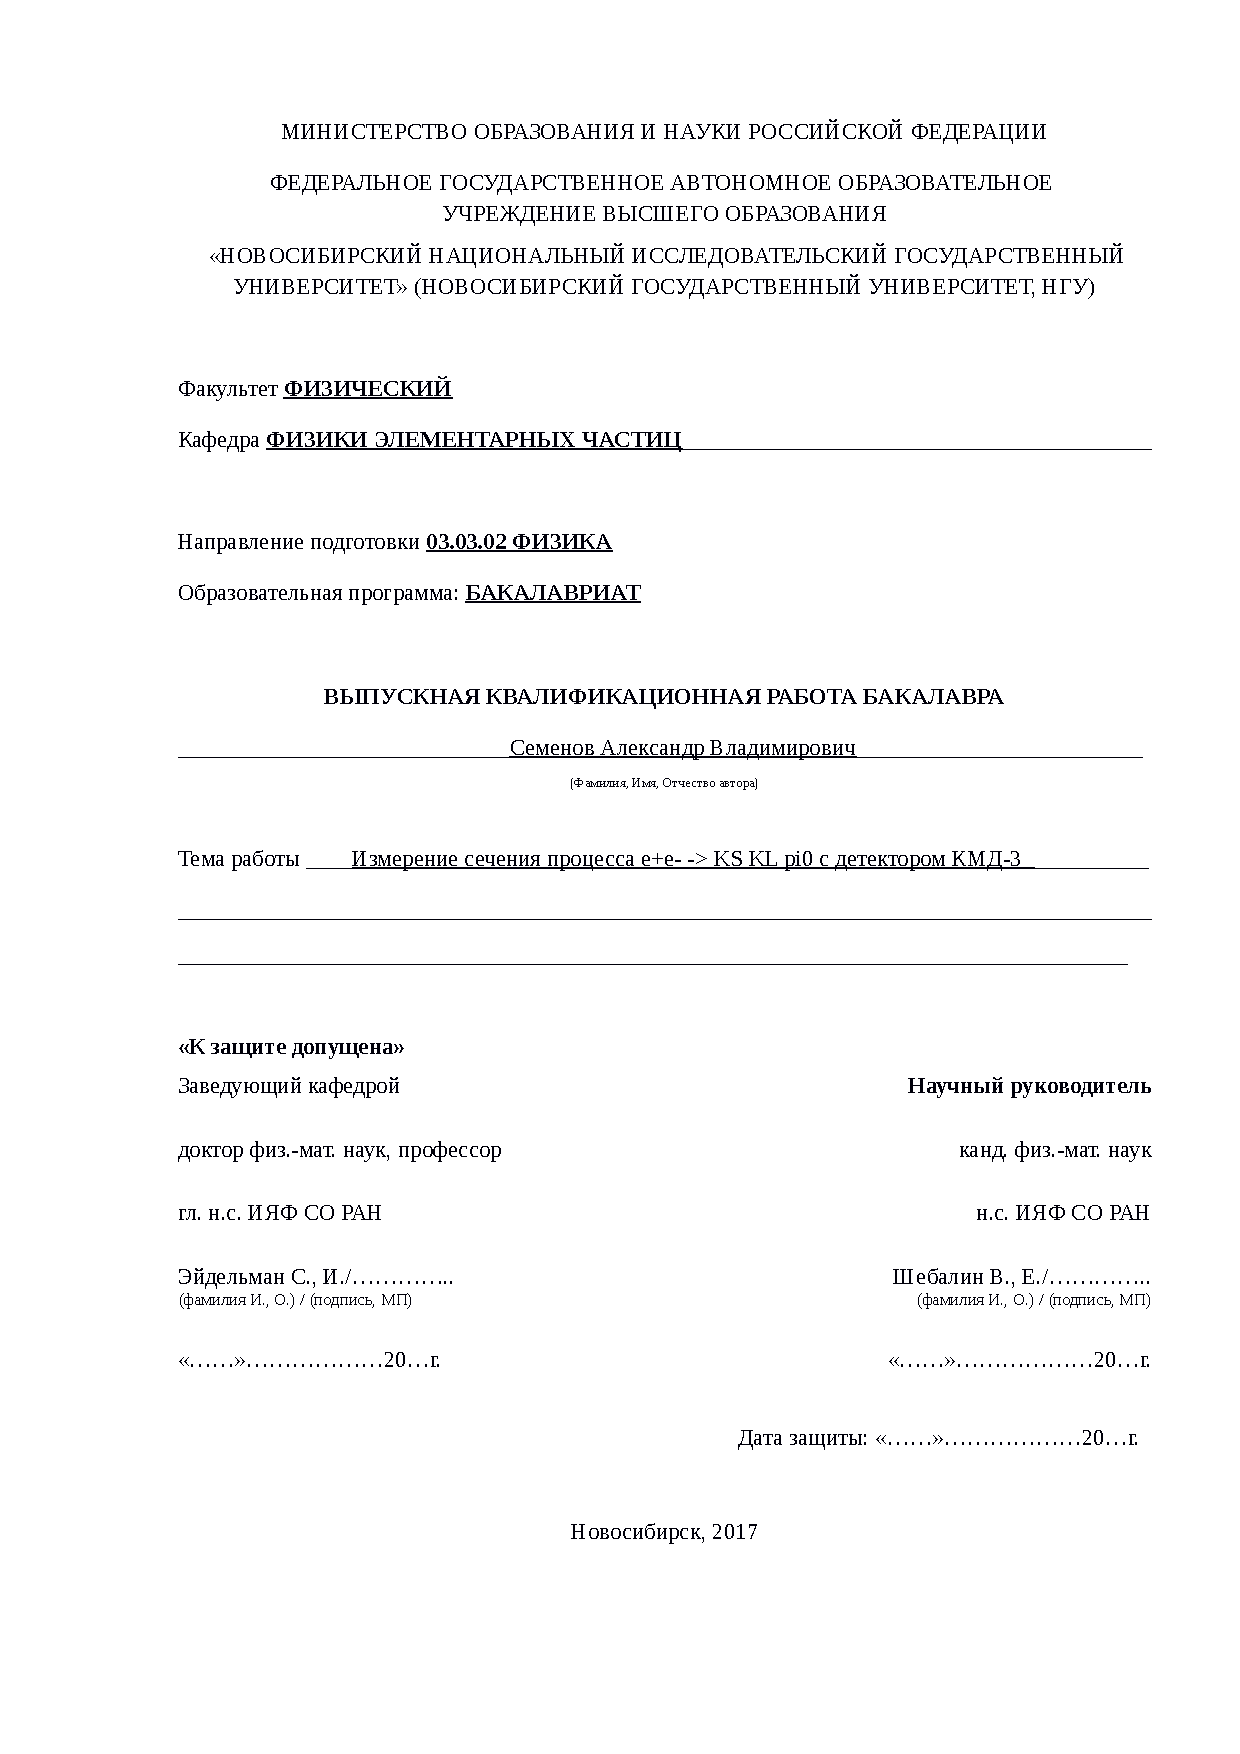
\includepdf{NSU/title}    % Титульный лист от НГУ
%% Ставим одинарный междустрочный интервал
\singlespacing
% Ставим геометрию для титульной страницы.
\newgeometry{left=3cm,right=1.5cm,top=2cm,bottom=2cm}

% Просто информация. Нигде в странице не используется, но зато попадёт в pdf info.
\author{Семенов А.\:В.}
\title{Измерение сечения e+ e- -> KS KL pi0}
\date{2017 г.}

\begin{titlepage}

%%%%%%%%%%%%%%%%%%%%%%%%%%%%%%%%%%%%%%%%%%%%%%%%%%%%%%%%%%%%%%%%%%%%%%%%%%%%%%%%

\begin{center}
    {\fnt{10.5} МИНИСТЕРСТВО ОБРАЗОВАНИЯ И НАУКИ РОССИЙСКОЙ ФЕДЕРАЦИИ} \\
        \vspace{0.3\baselineskip}
    {\fnt{10.5} ФЕДЕРАЛЬНОЕ ГОСУДАРСТВЕННОЕ АВТОНОМНОЕ ОБРАЗОВАТЕЛЬНОЕ \\ 
		\vspace{-0.3\baselineskip}
		УЧРЕЖДЕНИЕ ВЫСШЕГО ОБРАЗОВАНИЯ} \\
        \vspace{0.3\baselineskip}
    {\fnt{10.5} <<НОВОСИБИРСКИЙ НАЦИОНАЛЬНЫЙ ИССЛЕДОВАТЕЛЬСКИЙ ГОСУДАРСТВЕННЫЙ \\
		\vspace{-0.3\baselineskip}
		УНИВЕРСИТЕТ>> (НОВОСИБИРСКИЙ ГОСУДАРСТВЕННЫЙ УНИВЕРСИТЕТ, НГУ)}
\end{center}

%%%%%%%%%%%%%%%%%%%%%%%%%%%%%%%%%%%%%%%%%%%%%%%%%%%%%%%%%%%%%%%%%%%%%%%%%%%%%%%%

\vspace{0.5\baselineskip}

\noindent
{\fnt{11}Факультет}
$\overset{\text{\fnt{11}\textbf{ФИЗИЧЕСКИЙ}}\phantom{\hspace{10.9cm}}}{\underline{\hspace{0.88\textwidth}}}$

\vspace{0.3\baselineskip}

\noindent
{\fnt{11}Кафедра}
$\overset{\text{\fnt{11}\textbf{ФИЗИКИ ЭЛЕМЕНТАРНЫХ ЧАСТИЦ}}\phantom{\hspace{4.8cm}}}{\underline{\hspace{0.895\textwidth}}}$

\vspace{1\baselineskip}

\noindent
{\fnt{11}Направление подготовки}
$\overset{\text{\fnt{11}\textbf{03.03.02 ФИЗИКА}}\phantom{\hspace{8cm}}}{\underline{\hspace{0.73\textwidth}}}$

\vspace{0.3\baselineskip}

\noindent
{\fnt{11}Образовательная программа}
$\overset{\text{\fnt{11}\textbf{БАКАЛАВРИАТ}}\phantom{\hspace{7.3cm}}}{\underline{\hspace{0.69\textwidth}}}$

%%%%%%%%%%%%%%%%%%%%%%%%%%%%%%%%%%%%%%%%%%%%%%%%%%%%%%%%%%%%%%%%%%%%%%%%%%%%%%%%

\vspace{\baselineskip}

\begin{center}\bfseries
    {\fnt{11} ВЫПУСКНАЯ КВАЛИФИКАЦИОННАЯ РАБОТА БАКАЛАВРА} \\
\end{center}

%%%%%%%%%%%%%%%%%%%%%%%%%%%%%%%%%%%%%%%%%%%%%%%%%%%%%%%%%%%%%%%%%%%%%%%%%%%%%%%%

\vspace{0.3\baselineskip}

\noindent
$\overset{\text{\fnt{11}Семенов Александр Владимирович}}
{\underset{\text{\fnt{9}(фамилия, имя, отчество автора)}}{\underline{\hspace{\textwidth}}}}$

%%%%%%%%%%%%%%%%%%%%%%%%%%%%%%%%%%%%%%%%%%%%%%%%%%%%%%%%%%%%%%%%%%%%%%%%%%%%%%%%

\vspace{\baselineskip}

\noindent
{\fnt{11}Тема работы}
$\overset{\text{\fnt{11}Измерение сечения процесса e+e- -> KS KL pi0 с детектором КМД-3}}{\underline{\hspace{0.855\textwidth}}}$

\noindent
$\overset{}{\underline{\hspace{\textwidth}}}$

\noindent
$\overset{}{\underline{\hspace{\textwidth}}}$

%%%%%%%%%%%%%%%%%%%%%%%%%%%%%%%%%%%%%%%%%%%%%%%%%%%%%%%%%%%%%%%%%%%%%%%%%%%%%%%%

\vspace{2\baselineskip}

\noindent
\begin{tabular}{@{}p{0.5\textwidth}@{}@{}R{0.5\textwidth}@{}}
\fnt{11}\textbf{<<К защите допущена>>} &  \\
\fnt{11}Заведующий кафедрой,           & \fnt{11}\textbf{Научный руководитель} \\
\fnt{11}канд. физ.-мат. наук, доцент   & \fnt{11}канд. физ.-мат. наук, \\
\fnt{11}зав. лаб ИЯФ СО РАН            & \fnt{11}н.с. ИЯФ СО РАН\\
$\overset{\text{\fnt{11}Эйдельман, С.\,И.}}{\underset{\text{\fnt{8}(фамилия, И.\,О.)}}{\underline{\hspace{0.225\textwidth}}}}
\overset{\text{\fnt{11}/}}{}
\overset{\text{\fnt{11}}}{\underset{\text{\fnt{8}(подпись)}}{\underline{\hspace{0.125\textwidth}}}}$ &
$\overset{\text{\fnt{11}Шебалин, В.\,Е.}}{\underset{\text{\fnt{8}(фамилия, И.\,О.)}}{\underline{\hspace{0.225\textwidth}}}}
\overset{\text{\fnt{11}/}}{}
\overset{\text{\fnt{11}}}{\underset{\text{\fnt{8}(подпись)}}{\underline{\hspace{0.125\textwidth}}}}$ \\
$\overset{\text{\fnt{11}<<}}{}
\overset{\text{\fnt{11}}}{\underline{\hspace{0.05\textwidth}}}
\overset{\text{\fnt{11}>>}}{}
\overset{\text{\fnt{11}}}{\underline{\hspace{0.215\textwidth}}}
\overset{\text{\fnt{11}2017 г.}}{}$ & 
$\overset{\text{\fnt{11}<<}}{}
\overset{\text{\fnt{11}}}{\underline{\hspace{0.05\textwidth}}}
\overset{\text{\fnt{11}>>}}{}
\overset{\text{\fnt{11}}}{\underline{\hspace{0.215\textwidth}}}
\overset{\text{\fnt{11}2017 г.}}{}$ \\
& \\
& \fnt{11}\textbf{Консультант} \\
& \fnt{11}канд. физ.-мат. наук, \\
& \fnt{11}с.н.с. ИЯФ СО РАН\\
&
$\overset{\text{\fnt{11}Кардапольцев, Л.\,В.}}{\underset{\text{\fnt{8}(фамилия, И.\,О.)}}{\underline{\hspace{0.225\textwidth}}}}
\overset{\text{\fnt{11}/}}{}
\overset{\text{\fnt{11}}}{\underset{\text{\fnt{8}(подпись)}}{\underline{\hspace{0.125\textwidth}}}}$ \\
&
$\overset{\text{\fnt{11}<<}}{}
\overset{\text{\fnt{11}}}{\underline{\hspace{0.05\textwidth}}}
\overset{\text{\fnt{11}>>}}{}
\overset{\text{\fnt{11}}}{\underline{\hspace{0.215\textwidth}}}
\overset{\text{\fnt{11}2017 г.}}{}$
\end{tabular}

%%%%%%%%%%%%%%%%%%%%%%%%%%%%%%%%%%%%%%%%%%%%%%%%%%%%%%%%%%%%%%%%%%%%%%%%%%%%%%%%

\vspace{1.5\baselineskip}

\begin{flushright}
\fnt{11}
$\overset{\text{\fnt{11}Дата защиты: <<}}{}
\overset{\text{\fnt{11}}}{\underline{\hspace{0.05\textwidth}}}
\overset{\text{\fnt{11}>>}}{}
\overset{\text{\fnt{11}}}{\underline{\hspace{0.215\textwidth}}}
\overset{\text{\fnt{11}2017 г.}}{}$
\end{flushright}

%%%%%%%%%%%%%%%%%%%%%%%%%%%%%%%%%%%%%%%%%%%%%%%%%%%%%%%%%%%%%%%%%%%%%%%%%%%%%%%%

\vfill

\begin{center}
    \fnt{11} Новосибирск, 2017
\end{center}

\end{titlepage}

% Возвращаем всё назад: полуторный интервал и геометрию.
\onehalfspacing
\restoregeometry         % Титульный лист от НГУ
%\chapter*{Аннотация}


% Оглавление (ГОСТ Р 7.0.11-2011, 5.2)
\pagenumbering{gobble}
\tableofcontents
\thispagestyle{empty}
        % Оглавление
%\chapter*{Введение}							% Заголовок
\addcontentsline{toc}{chapter}{Введение}	% Добавляем его в оглавление

\newcommand{\actuality}{}
\newcommand{\aim}{\textbf{Целью}}
\newcommand{\tasks}{задачи}
\newcommand{\defpositions}{\textbf{Основные положения, выносимые на~защиту:}}
\newcommand{\novelty}{\textbf{Научная новизна}}
\newcommand{\influence}{\textbf{Научная и практическая значимость}}
\newcommand{\reliability}{\textbf{Степень достоверности}}
\newcommand{\probation}{\textbf{Апробация работы.}}
\newcommand{\contribution}{\textbf{Личный вклад.}}
\newcommand{\publications}{\textbf{Публикации.}}

{\actuality}
Данная работа посвящена разработке рентгенооптических трактов синхротронного источника СКИФ --- <<Сибирский кольцевой источник фотонов>>. За последние три десятилетия мир увидел активное развитие специализированных источников синхротронного излучения и соответствующих методов исследования вещества с использованием синхротронного излучения в рентгеновском диапазоне. Главные параметры излучения, который достигаются на данных установках является высокий поток фотонов, направленность излучения в малый телесный угол, когерентность. Эти параметры крайне необходимы для проведения качественных экспериментов с революционными результатами в области химии, биологии, материаловедении, медицины и многих других отраслях науки и техники.

Высокая востребованность данной работы заключается в том, что в отечественной науке наблюдается стагнация в области развития специализированных источников рентгеновского излучения. Проектируемый в Новосибирске синхротронный источник является первым на территории России специализированным источником с проектными параметрами не уступающими мировым установкам, а по некоторым данным с запасом превосходящих их, такие, например, как: MAX-IV, NSLS-II, PETRA-III, Diamond и д.р.

\textbf{Цель} данной работы --- разработка проекта станций первой очереди, вставными устройствами на которых являются сверхпроводящие ондуляторы. Это станции: 1-1 --- <<Микрофокус>>, 1-2 --- <<Структурная диагностика>>, 1-4 --- <<XAFS-спектроскопия и магнитный дихроизм>>.  

В цели проектирования входит ряд \textbf{задач}:
\begin{itemize}

	\item Расчёт ондуляторного излучения с помощью численного моделирования, получение спектров и сечений пучка из указанных устройств, максимально обективно описывающих реальное излучение.
	\item Разработка оптических трактов: расчёт тепловых нагрузок, расчёт спектров и сечений пучка после прохождение оптических элементов. 
	\item Разработка программного кода для реализации выше приведённых задач и удобному воспроизведению результатов расчётов любым участником проекта.

\end{itemize} % Характеристика работы по структуре во введении и в автореферате не отличается (ГОСТ Р 7.0.11, пункты 5.3.1 и 9.2.1), потому её загружаем из одного и того же внешнего файла, предварительно задав форму выделения некоторым параметрам

%% регистрируем счётчики в системе totcounter
\regtotcounter{totalcount@figure}
\regtotcounter{totalcount@table}       % Если поставить в преамбуле то ошибка в числе таблиц
\regtotcounter{TotPages}               % Если поставить в преамбуле то ошибка в числе страниц

%% на случай ошибок оставляю исходный кусок на месте, закомментированным
%Полный объём диссертации составляет  \ref*{TotPages}~страницу с~\totalfigures{}~рисунками и~\totaltables{}~таблицами. Список литературы содержит \total{citenum}~наименований.
%
    % Введение
%\input{part1}           % Глава 1
%\input{part2}           % Глава 2

%\input{part3}           % Глава 3
\chapter{Теоретической обоснование используемых численных методов}
\section{Излучение релятивистской электрона в синусоидальном магнитном поле}
В этой части мы дадим вывод излучения релятивистского электрона в $r\omega$-пространстве, движущегося в синусоидальном магнитном поле. Единственно приближение, которым мы будем пользоваться, --- прааксиальное приближение. Вывод интересен тем, что даёт наглядное представление о спектре частицы, угловом распределении интенсивности в зависимости от резонансной частоты. В заключении главы, будет приведён вывод распределения электромагнитного поля(в ближней зоне???) через потенциалы Лиенара-Вихерта, будет получен результат, который даст представление о методах используемых в численных симуляциях, на примере кода SRW. В наших рассуждениях мы следовали (Салдин Гелони)
\subsection{Уравнение движения электрона в ондуляторе}
Выведем спектр излучения из ондулятора. Вывод начнём с уравнения движение релятивистского электрона в магнитном поле.

\begin{equation}
	\vec{F} = e[\vec{v} \times \vec{B}],
\end{equation} 
где $e$ --- заряд электрона, а $\vec{v}$ и $\vec{B}$ скорость частицы и магнитное поле соответственно. Уравнение можно переписать в виде:

\begin{equation}
	\cfrac{d\vec{p}}{dt} = \cfrac{e}{\gamma m_e}[\vec{v} \times \vec{B}],
\end{equation}
где $\gamma$ --- лоренц фактор, появившийся из релятивистского импульса. Направим ось $z$ вдоль направления релятивистского движения электрона и введём магнитное поле в ондуляторе $B_0\cos(k_w z)$, направленное вдоль оси $y$, где $k_w$ связана с периодом ондулятора следующим образом $k_w = 2\pi/\lambda_w$. 

\begin{equation}
	\label{eq:eq_of_motion}
	\begin{cases}
		\cfrac{d^2 x}{dt^2} = - \cfrac{e B_0}{\gamma m_e}\cfrac{dz}{dt} \cos(k_w z)\\
		\cfrac{d^2 z}{dt^2} = \cfrac{e B_0}{\gamma m_e}\cfrac{dx}{dt} \cos(k_w z)
	\end{cases} 
\end{equation}

один раз интегрируя первой уравнение из системы с заменой $dz = \beta cdt$, где $\beta = \|\vec{v}\| /c$, можно получить: 

\begin{equation}
 	\label{eq:dx/dt}
	\cfrac{dx}{dt} = - \cfrac{eB_0}{\gamma m_ek_w} \sin(k_w z)
\end{equation}
Введём коэффициент ондуляторности --- $K = \cfrac{eB_0 \lambda}{2\pi m_ek_w}$, который показывает угол отклонения электрона от оси $z$(?????). 

Подставляя получившийся результат~\ref{eq:dx/dt} во второе уравнение системы~\ref{eq:eq_of_motion} и интегрируя с пределами интегрирования от $0$ до некоторого $z_0$, получим систему:

\begin{equation}
	\begin{cases}
	\label{eq:eq_of_motion_velocity}
		\cfrac{dx}{dt} = - \cfrac{Kc}{\gamma} \sin(k_w z)\\
		\cfrac{dz}{dt} = \beta c - \cfrac{K^2 c}{2 \gamma^2 \beta}\sin^2(k_w z)
	\end{cases} 
\end{equation}

Проинтегрировав оба уравнения(в каких пределах?), получим (Wiedemann),

\begin{equation}
	\begin{cases}
	\label{eq:eq_of_motion_trej}
		x = \cfrac{Kc}{с\gamma k_w \beta} \cos(k_w\overline{\beta}ct)\\
		z = \overline{\beta}ct + \cfrac{K^2}{8 \beta^2 \gamma^2 k_w}\sin(2k_w\overline{\beta}ct), 
	\end{cases} 
\end{equation}
где был введено обозначение $\overline{\beta}$, которое определяется как $\overline{\beta}c = \beta c(1 - \cfrac{K^2}{4 \beta^2 \gamma^2})$
Из~\ref{eq:eq_of_motion_velocity} видно, что продольная скорость испытывает о осцилляции с удвоенной частотой...
\subsection{Решение волнового уравнения в прааксиальном приближении}
Вывод спектра излучения будем проводить в $r\omega$-пространстве. Начнём с уравнений Максвелла в вакууме:
\begin{equation}
	\begin{cases}
		\nabla \cdot \vec{E} = 4\pi \rho\\
		\nabla \cdot \vec{E} = 0\\
		[\nabla \times \vec{E}] = -\cfrac{1}{c} \cfrac{d\vec{B}}{dt}\\
		[\nabla \times \vec{B}] = \cfrac{4\pi}{c} \vec{j} + \cfrac{1}{c} \cfrac{\partial\vec{E}}{\partial t}
	\end{cases} 
\end{equation}
Из уравнений тривиально можно получить неоднородное волновое уравнение(какая калибровка?): 
\begin{equation}
	\label{eq:inhomo_wave_eq_xt}
	\pdv[2]{\vec{E}}{t} + c^2 \nabla^2 \vec{E} = 4\pi c^2 \nabla \rho + 4\pi \pdv{\vec{j}}{t}
\end{equation}
Это же уравнение перепишем в $r\omega$-пространстве, определив преобразование Фурье следующим образом:
\begin{equation}
	\label{eq:Fourier_wt}
	\begin{array}{lcl}
		\vec{\widetilde{E}}(r, \omega) = \displaystyle\int\limits_{-\infty}^{\infty} dt \vec{E}(r, t)\exp[-i\omega t]\\
		\\
		\vec{E}(r, \omega) = \cfrac{1}{2\pi}\displaystyle\int\limits_{-\infty}^{\infty} d\omega \vec{\widetilde{E}}(r, t)\exp[i\omega t]
	\end{array}
\end{equation}
Применив к уравнению~\ref{eq:inhomo_wave_eq_xt}, получим:
\begin{equation}
	\omega^2 \vec{\widetilde{E}} + c^2 \nabla^2 \vec{\widetilde{E}} = 4\pi c^2 \nabla  \widetilde{\rho} - 4i\pi\omega\vec{\widetilde{j}}
\end{equation}
Перепишем это уравнение в приближении медленно меняющейся амплитуды в сравнение с частотой осцилляций, что есть $\vec{\widetilde{E}} =  \vec{\overline{E}}\exp[i\omega z/c]$, в приближении $\cfrac{\partial |E|}{\partial z} \ll \cfrac{\omega}{c}|E|$. Где временная зависимость разложена до нулевого порядка малости, исходя из уравнения~\ref{eq:eq_of_motion_trej}. Получим:
\begin{equation}
	\label{eq:wave_slow_vary}
	c^2\bigg(\nabla^2 \vec{\widetilde{E}} - \cfrac{2i\omega}{c}\pdv{\vec{\widetilde{E}}}{z}\bigg)\exp[i\omega z/c] = 4\pi c^2 \nabla  \widetilde{\rho} - 4i\pi\omega\vec{\widetilde{j}}
\end{equation}

Для электрона движущегося в вакууме ток и плотность заряда выражается через дельта-функцию Дирака:

\begin{equation}
	\begin{array}{lcl}
		\rho(r,t) = -e\delta(\vec{r}- \vec{r'}(t)) = -\cfrac{e}{v_z(z)}\delta(\vec{r}_{\bot}- \vec{r'}_{\bot}(z))\delta(\cfrac{s(z)}{v} - t)\\
		\vec{j}(r,t) = \vec{v}\rho(r,t)	
	\end{array}
\end{equation} 
В $r\omega$-пространстве: 
\begin{equation}
	\begin{array}{lcl}
		\widetilde{\rho}(r,\omega) = -\cfrac{e}{v_z(z)}\delta(\vec{r}_{\bot}- \vec{r'}_{\bot}(z))\exp[\cfrac{iws(z)}{v}]\\
		\widetilde{\vec{j}}(r,\omega) = \vec{v}\widetilde{\rho}(r,\omega)	
	\end{array}
\end{equation} 
Подставим фурье-образы плотности тока и заряда в уравнение~\ref{eq:wave_slow_vary}, (где производная по градиентному члену? добавить это)
\begin{equation}
	\label{eq:wave_eq}
	\begin{array}{lcl}
		\nabla^2 \vec{\widetilde{E}} - \cfrac{2i\omega}{c}\cfrac{\partial\vec{\widetilde{E}}}{\partial z} = 
		\cfrac{4\pi e}{v_z(z)} \exp[iw\bigg(\cfrac{s(z)}{v} - \cfrac{z}{c}\bigg)]
		\bigg(  
			\cfrac{i\omega}{c^2}\vec{v}(z)
			-\nabla\bigg) \delta(\vec{r}_{\bot} - \vec{r'}_{\bot}(z)) 
		
	\end{array}
\end{equation} 
Получившиеся уравнение является точным. Теперь мы можешь применить параксиальное приближении. 
\begin{equation}
	\label{eq:wave_slow_vary_parax}
	\begin{array}{lcl}
		\nabla_{\bot}^2 \vec{\widetilde{E}}_{\bot} - \cfrac{2i\omega}{c}\cfrac{\partial\vec{\widetilde{E}}_{\bot}}{\partial z} = 
		\cfrac{4\pi e}{v_z(z)} \exp[iw\bigg(\cfrac{s(z)}{v} - \cfrac{z}{c}\bigg)]\bigg(  
			\cfrac{i\omega}{c^2}\vec{v}_{\bot}(z) 
			-\nabla_{\bot}\bigg) \delta(\vec{r}_{\bot} - \vec{r'}_{\bot}(z)) 
	\end{array}
\end{equation} 
Вторая производная по z, появляющаяся из оператора Лапласа полагается много меньшим по сравнению с первой производной по $z$ в уравнении~\ref{eq:wave_slow_vary_parax} исходя из предположения медленно меняющейся амплитуды.

Перед нами неоднородное дифференциальное уравнение в частных производных, которое решается с помощью функции Грина. Для дифференциального оператора $\partial_t - k\nabla_{2D}^2$ функция Грина есть: $\cfrac{1}{4\pi kt}\exp[-\rho^2/4kt]$. В частности для уравнения~\ref{eq:wave_slow_vary_parax}
\begin{equation}
	\label{eq:Green_func}
	G(z_0 - z'; \vec{r}_{\bot 0} - \vec{r'}_{\bot}) = 
	- \cfrac{1}{4\pi (z_0 - z')}\exp[i\omega \cfrac{|\vec{r}_{\bot 0} - \vec{r'}_{\bot}|^2}{2c(z_0 - z')}]
\end{equation} 
Получим решение для функции распределения поля:

\begin{equation}
	\begin{array}{lcl}
		\vec{\widetilde{E}}_{\bot}(z_0,  \vec{r}_{\bot 0}, \omega) = -\cfrac{e}{c}  \displaystyle\int\limits_{-\infty}^{\infty}\int\limits_{-\infty}^{\infty} dz'd\vec{r'}\cfrac{1}{z_0 - z'}
		\bigg(\cfrac{i\omega}{c^2}\vec{v}_{\bot}(z')
		-\nabla'_{\bot}\bigg) \delta(\vec{r'}_{\bot} - \vec{r'}_{\bot}(z'))\times\\
		\exp[iw\bigg( \cfrac{|\vec{r}_{\bot 0} - \vec{r'}_{\bot}|^2}{2c(z_0 - z')} +\cfrac{s(z')}{v} - \cfrac{z'}{c} \bigg)]
	\end{array}	
\end{equation}
Проинтегрировав по $d\vec{r'}$ получим общее решение уравнения~\ref{eq:wave_eq} :
\begin{equation}
	\label{eq:field_in_parax}
	\begin{array}{lcl}
		\vec{\widetilde{E}}_{\bot}(z_0,  \vec{r}_{\bot 0}, \omega) = -\cfrac{i\omega e}{c^2}  \displaystyle\int\limits_{-\infty}^{\infty} dz'
		\cfrac{1}{z_0 - z'}
		\bigg(\cfrac{\vec{v}_{\bot}(z')}{c}
		- \cfrac{\vec{r}_{\bot 0} - \vec{r'}_{\bot}(z')}{(z_0 - z')}\bigg)\times\\
		\exp[iw\bigg(\cfrac{|\vec{r}_{\bot 0} - \vec{r'}_{\bot}(z')|^2}{2c(z_0 - z')} + \cfrac{s(z')}{v} - \cfrac{z'}{c} \bigg)]
	\end{array}	
\end{equation}
Что есть распределение электромагнитного поля в точке наблюдения $\vec{r}_0$.

\subsection{Излучение планарного ондулятора}
В этой секции мы рассмотрим излучение планарного ондулятора использую наши предыдущие результаты~\ref{eq:field_in_parax} и~\ref{eq:eq_of_motion_trej}. Сперва проанализируем получившиеся распределение поля~\ref{eq:field_in_parax}: в случае ондулятора, член $(z_0 - z')^{-1}$ можно разложить около точки $z'$, так как размер ондулятора много меньше чем расстояние, с которого мы наблюдаем излучение: $\lambda_w N \ll z_0$, где $N$ число периодов ондулятора.

Воспользовавшись решениями~\ref{eq:eq_of_motion_velocity} и~\ref{eq:eq_of_motion_trej} и помня $\vec{r}_{\bot 0}/z_0 = \vec{\theta}$ преобразуем уравнение~\ref{eq:field_in_parax} к виду:
\begin{equation}
	\label{eq:field_in_parax}
	\begin{array}{lcl}
		\vec{\widetilde{E}}_{\bot}(z_0,  \vec{r}_{\bot 0}, \omega) =
		\cfrac{i\omega e}{c^2z_0} \exp[i\cfrac{\omega \theta^2 z_0}{2c}]
	 	\displaystyle\int\limits_{-\lambda_w N/2}^{\lambda_w N/2} dz'\exp[i\Phi_T]
		\bigg(\cfrac{K}{\gamma}\sin(k_w z)\vec{e_x} + \vec{\theta}\bigg)
	\end{array}	
\end{equation}
Здесь мы отбросили члены первого и большего порядка малости по $1/z_0$. Где за $\Phi_T$ мы обозначили:
\begin{equation}
	\Phi_T = 
	\bigg(\cfrac{\omega}{2c\widetilde{\gamma}^2} + 
	\cfrac{\omega\vec{\theta}^2}{2c}\bigg)z' - 
	\cfrac{K^2}{8\gamma^2}\cfrac{\omega}{k_w c}\sin(2k_wz') - \cfrac{K{\theta_x}}{\gamma}\cfrac{\omega}{k_w c}\cos(k_w z'),
\end{equation}
где $\widetilde{\gamma} = \cfrac{\gamma}{\sqrt{1 + K^2/2}}$.

Пределы интегрирования ограничили по длиной ондулятора от $-\lambda_w N/2$ до $\lambda_w N/2$, считая вклад в излучение от ондулятора доминирующим надо остальными вкладами от соответствующих участков траектории. На это шаге уже можно заметить, что излучение на оси будет линейно поляризованно, это есть вклад члена с током, вклад же плотности заряда или градиентный член, даёт вариацию поляризации, при наблюдении под некоторым углом $\theta$ к оси.

Если переписать~\ref{eq:field_in_parax} в следующе виде:
\begin{equation}
		\label{eq:field_in_parax_Bessel}
		\begin{array}{lcl}
			\vec{\widetilde{E}}_{\bot}(z_0,  \vec{r}_{\bot 0}, \omega) =
			\cfrac{i\omega e}{c^2z_0} \exp[i\cfrac{\omega \theta^2 z_0}{2c}]
			\displaystyle\sum_{m,n=-\infty}^{+\infty}
			J_m\bigg(-\cfrac{K^2}{8\gamma^2}\cfrac{\omega}{k_w c}\bigg)
			J_n\bigg(-\cfrac{K{\theta_x}}{\gamma}\cfrac{\omega}{k_w c}\bigg)\times\\
			\exp[\cfrac{i\pi n}{2}]
			\displaystyle\int\limits_{-\lambda_w N/2}^{\lambda_w N/2} dz'\exp[i(2m + n)k_wz']
			\bigg(\cfrac{K}{2i\gamma}\big(\exp[2ik_w z'] - 1\big)\vec{e_x} + \vec{\theta}\exp[ik_w z']\bigg)\times\\
			\exp[i\bigg(k_w \cfrac{\Delta\omega}{\omega_r} + 
			\cfrac{\omega\vec{\theta}^2}{2c}\bigg)z'],
		\end{array}	
\end{equation}
Где мы ввели $\omega = \omega_r + \Delta\omega$, $\omega_r = 2c\widetilde{\gamma}^2k_w$ и использовали формулу Якоби — Ангера:
\begin{equation}
	\begin{array}{lcl}
		\exp[iz\cos(\theta)] = 
		\displaystyle\sum\limits_{n =-\infty}^{\infty}
		i^n J_n(z)\exp[in\theta]\\	
		\exp[iz\sin(\theta)] = 
		\displaystyle\sum\limits_{n =-\infty}^{\infty}
		J_n(z)\exp[in\theta]
	\end{array}	
\end{equation}




До сих пор мы пользовались только двумя приближениями, --- медленно меняющейся амплитудой и параксиальным приближением, теперь можем воспользоваться следующим параметром --- количеством периодов ондулятора, --- $N$. Для этого обратим внимание на первой слагаемое в фазовом множителя под интегралом, и заметим, что если $k_w \cfrac{\Delta\omega}{\omega_r} + 
\cfrac{\omega\vec{\theta}^2}{2c} \ll k_w$, то фаза меняется медленно на одном периоде и эта фаза не занулит интеграл. Отметим, что для резонанса условия должны выполняться по отдельности, т.е. $\cfrac{\Delta\omega}{\omega_r} \ll 1$ и $\cfrac{\omega\vec{\theta}^2}{2c} \ll 1$, последнее даёт углы наблюдения вблизи резонанса: $\theta^2 \ll \cfrac{1}{\widetilde{\gamma}^2}$. Теперь необходимо обратить внимание на аргументы функций Бесселя, а именно: 
\begin{equation}
	\begin{array}{lcl}
		u = -\cfrac{K^2}{8\gamma^2}\cfrac{\omega}{k_w c}\\
		v = -\cfrac{K{\theta_x}}{\gamma}\cfrac{\omega}{k_w c} = - \cfrac{K{\theta_x}}{\gamma}
		\bigg(1 + \cfrac{\Delta\omega}{\omega_r}\bigg)2\widetilde{\gamma}^2 \lesssim
		\cfrac{2K{\theta_x}\widetilde{\gamma}}{\sqrt{1 + K^2/2}} \lesssim \theta_x\widetilde{\gamma} \ll 1
	\end{array}	
\end{equation}
Зная, что $J_\alpha(x) \thicksim \displaystyle\sum\limits_{n =0}^{\infty} x^{2\beta + \alpha} $, видим, что вклад нулевого порядка по $\theta_x\widetilde{\gamma}$, т.е. $J_\alpha(x) \thicksim 1$ даёт только функция Бесселя с индексом $n = 0$. Здесь мы пока не учитываем градиентный член пропорциональный $\vec{\theta}$, таким образом из оставшихся фазовых множителей можно выписать условия на индекс $m$. Они определяются нулями в аргументах соответствующих фаз или $m = -1$ и $m = 0$, оба оставшихся члена пропорциональны $\cfrac{K}{\gamma}$. 

Теперь вернёмся к градиентному члену, вклад от которого занулиться при усреднении по длине ондулятора при $n = 0$, этот вклад даст ненулевой вклад при $n = 1 - 2m$, т.о. в ход пойдут следующие члены разложения $J_m(v)$. Однако, помня интересующий нас диапазон углов, члены разложения будут порядка $\theta_x v^m$, очевидно, что их вклады пренебрежимо малы по сравнению с вкладами токового члена $\vec{e}_x$. Учитывая выше сказанные приближения, перепишем~\ref{eq:field_in_parax_Bessel}
\begin{equation}
	\label{eq:field_dist_in_integral}
	\begin{array}{lcl}
		\vec{\widetilde{E}}_{\bot}(z_0,  \vec{r}_{\bot 0}, \omega) =
		\cfrac{\omega e}{2c^2z_0}\cfrac{K}{\gamma}\exp[i\cfrac{\omega \theta^2 z_0}{2c}]
		\bigg(J_1(v) - J_0(v)\bigg)\vec{e}_x\times\\
		\\
		\displaystyle\int\limits_{-\lambda_w N/2}^{\lambda_w N/2} dz'
		\exp[i\bigg(k_w \cfrac{\Delta\omega}{\omega_r} + 
		\cfrac{\omega\vec{\theta}^2}{2c}\bigg)z'],
	\end{array}	
\end{equation}
Интеграл легко берётся:
\begin{equation}
	\label{eq:field_dist_nonNorm}
	\begin{array}{lcl}
		\vec{\widetilde{E}}_{\bot}(z_0,  \vec{r}_{\bot 0}, \omega) =
		\cfrac{\omega eL}{c^2z_0}\cfrac{K}{\gamma}\exp[i\cfrac{\omega \theta^2 z_0}{2c}]
		\sinc[\bigg(k_w \cfrac{\Delta\omega}{\omega_r} + 
		\cfrac{\omega\vec{\theta}^2}{2c}\bigg)L/2]\vec{e}_x ,
	\end{array}	
\end{equation}
где введено обозначение: $A_{JJ} = J_1(v) - J_0(v)$. 

В следующем параграфе мы займёмся выводном влияния конченого эмиттанса на распределение излучения, чтобы облегчить выкладки мы введём нормализованные единицы.
\begin{equation}
	\label{eq:norm_units}
	\begin{array}{lcl}
		\hat{E}_{\bot} = \cfrac{c^2z_0\gamma \widetilde{E}_{\bot}}{e\omega KLA_{JJ}}\\
		\hat{\theta} = \theta\sqrt{\cfrac{\omega L}{c}}\\
		\hat{z} = \cfrac{z}{L} ,
	\end{array}	
\end{equation}
а также, 
\begin{equation}
	\hat{C} = CL = 2\pi N\cfrac{\Delta\omega}{\omega_r}
\end{equation}
Теперь уравнения~\ref{eq:field_dist_nonNorm} и~\ref{eq:field_dist_in_integral} могут быть переписаны в нормализованных единицах.
\begin{equation}
	\label{eq:field_dist_in_integral}
	\begin{array}{lcl}
		\hat{E}_{\bot} = e^{i\Phi}
		\displaystyle\int\limits_{-1/2}^{1/2} dz'
		\exp[i\bigg(\hat{C} + 
		\cfrac{\hat{\theta}^2}{2}\bigg)z'],
	\end{array}	
\end{equation}

\begin{equation}
	\label{eq:field_dist_Norm}
	\begin{array}{lcl}
		\hat{E}_{\bot} = e^{i\Phi}
		\sinc\bigg(\cfrac{\hat{C}}{2} + 
		\cfrac{\hat{\theta}^2}{4}\bigg),
	\end{array}	
\end{equation}
\begin{figure}
	\centering  
	\begin{minipage}{0.49\textwidth}
		\centering
		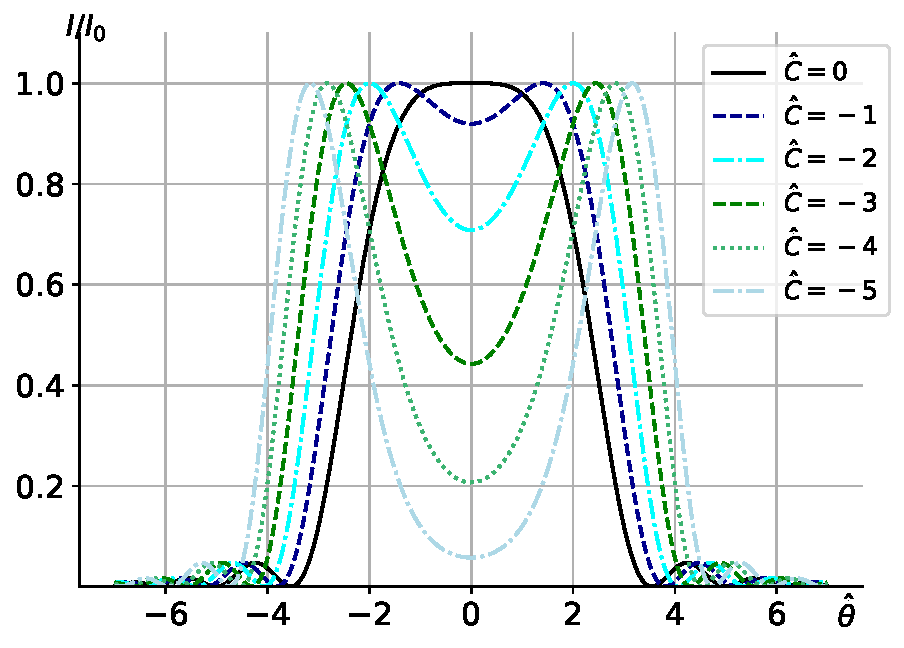
\includegraphics[width=\textwidth]{pic/angleC_neg.pdf}
		\caption{}
		\label{fig:angle_dist_C_neg}
	\end{minipage}\hfill
	\begin{minipage}{0.49\textwidth}
		\centering
		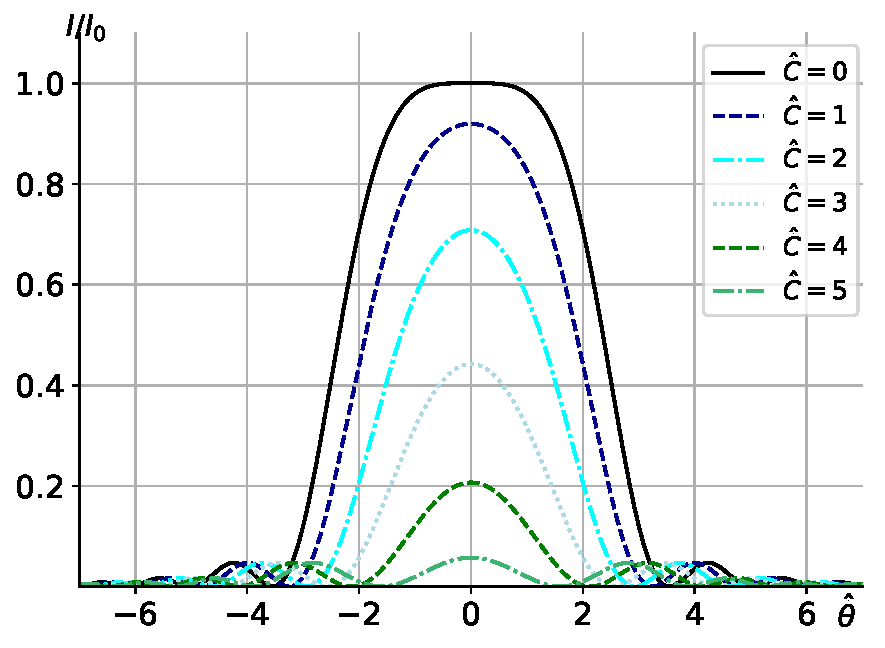
\includegraphics[width=\textwidth]{pic/angleC_pos.pdf}
		\caption{}
		\label{fig:angle_dist_C_pos}
	\end{minipage}    
\end{figure}
На рис.~\ref{fig:angle_dist_C_neg} и рис.~\ref{fig:angle_dist_C_pos} изображены угловые распределения излучения. Из них можно понять, что если сдвижка по спектру идёт в область меньших частот, то условие резонанса удовлетворяется на других углах и проинтегрированные по даст некоторую интенсивность. Если же сдвигаться по спектру в область более высоких частот, что условие резонанса на углах не будет выполняться и интенсивность быстро упадёт. На рис.~\ref{fig:spec_integrate_angle} представлен проинтегрированный по углам $\hat{\theta}$ спектр.
\begin{figure}[htbp]
	\centering
	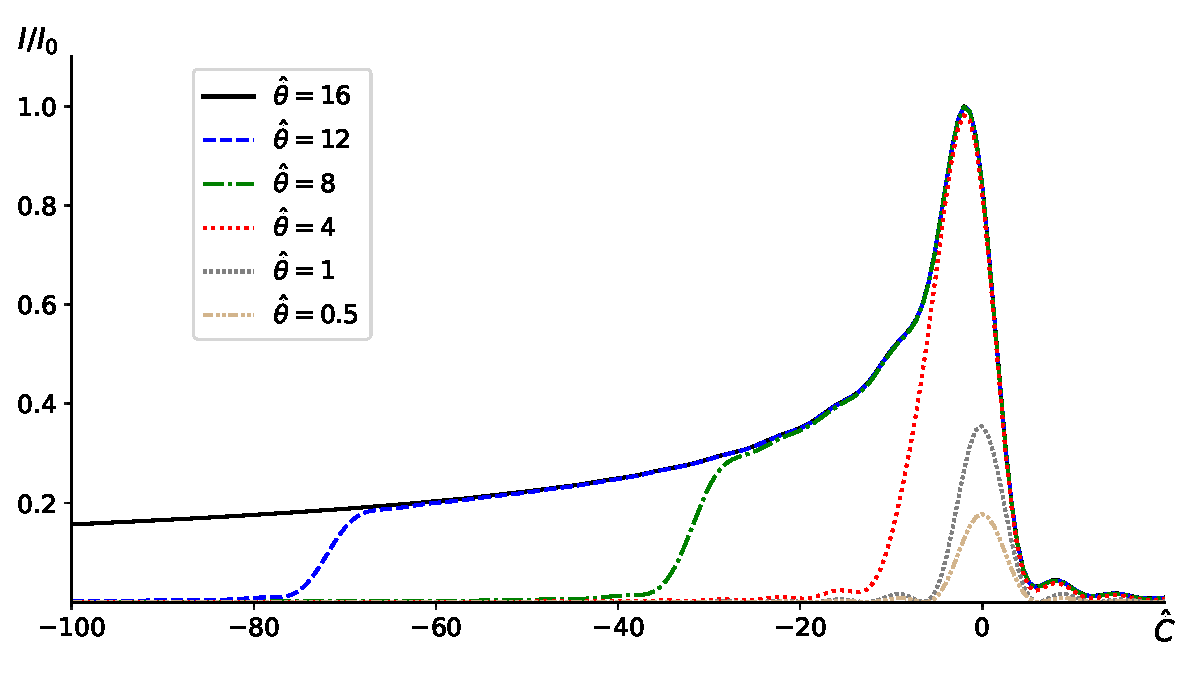
\includegraphics[width=.99\textwidth]{{pic/spec_integ_ang}.pdf}
	\caption{} 
	\label{fig:spec_integrate_angle}
\end{figure}

\subsection{Излучение клинообразного ондулятора}
В этой секции мы рассмотрим излучение из ондулятора специальной конструкции, который может дать широкий спектр. Идея в том, что разбить ондулятор на несколько секций с различным $K$ в каждой из них. Такая расстановка в первом приближении должна дать набор резонансов, которые должны сложиться в один сплошной спектр. Более детальное рассмотрение покажет, что в зависимости от корреляции фазы электрона между этими сегментами, могут проявляться интерференционные эффекты, которые в значительной степени будут изменять форму спектра. В нашем рассмотрении мы покажем влияние указанных вкладов для случая скачкообразного изменения поля, а также для классического случая клинообразного, т.н. зарубежной литературе tapered undulator.

Свои выкладки начнём с модифицированного интеграла~\ref{eq:field_dist_in_integral}, 
\begin{equation}
	\begin{array}{lcl}
	\vec{\widetilde{E}}_{\bot}(z_0,  \vec{r}_{\bot 0}, \omega) =
	\cfrac{\omega eA_{JJ}}{2c^2z_0}\cfrac{K}{\gamma}
	\displaystyle\int\limits_{-\lambda_w N/2}^{\lambda_w N/2} dz'
	\exp[iCz'] 	\vec{e}_x,
	\end{array}	
\end{equation} 
Здесь, для краткости выкладок, излучения мы сморим на оси, т.е. $\theta = 0$. В случае секционного ондулятора коэффициент ондуляторности меняется вдоль ондулятора, поэтому $K = K_0 + n\Delta K$, а также $C = C_0 + n\Delta C$, где $n$ --- это номер секции. $\Delta {C}$ введено следующим образом, помня $\omega_r = 2c\widetilde{\gamma}^2k_w$:
\begin{equation}
	C =k_w\cfrac{\Delta \omega}{\omega_r} = \cfrac{\Delta \omega_r}{2c\gamma}\bigg(1 + \cfrac{(K_0 + n\Delta K)^2}{2}\bigg) \approx \cfrac{\Delta \omega_r}{2c\gamma}\bigg(1 + \cfrac{K^2_0}{2}(1 + \cfrac{n\Delta K}{K_0})\bigg) = C_0 + \Delta C
\end{equation} 
Секций, для условности, мы возьмём пять, и для удобства нумерацию будем вести $-2, -1, ... , 2$. Поэтому интеграл перепишеться в виде:
\begin{equation}
	\begin{array}{lcl}
	\vec{\widetilde{E}}_{\bot}(z_0,  \vec{r}_{\bot 0}, \omega) =
	\cfrac{\omega eA_{JJ}}{2c^2 \gamma z_0}
	\displaystyle\sum\limits_{n =-2}^{2}(K_0 + n\Delta K)
	\displaystyle\int\limits_{(2n + 1)L_s/2}^{(2n - 1)L_s/2} dz'
	\exp[i(C_0 + n\Delta C)z']	\vec{e}_x,
	\end{array}	
\end{equation} 
Взяв интеграл, получим:
\begin{equation}
	\begin{array}{lcl}
	\vec{\widetilde{E}}_{\bot}(z_0,  \vec{r}_{\bot 0}, \omega) =
	\cfrac{\omega eA_{JJ}}{2c^2 \gamma z_0}
	\displaystyle\sum\limits_{n =-2}^{2}(K_0 + n\Delta K)
	\sinc(\hat{C}/2)e^{in({C}_0 + n\Delta {C})L}	\vec{e}_x,
	\end{array}	
\end{equation} 
Возведя в квадрат получим интенсивность:
\begin{equation}
	\begin{array}{lcl}
	{\widetilde{I}} =
	\bigg(\cfrac{\omega eA_{JJ}}{2c^2 \gamma z_0}\bigg)^2\bigg[
	\displaystyle\sum\limits_{n =-2}^{2}(K_0 + n\Delta K)^2\sinc^2(\hat{C_0} + n\Delta \hat{C}/2) + \\
		
	\displaystyle\mathop{\sum\limits_{n, m =-2}^{2}}_{n \neq m}K^2_0\bigg(1 + n\cfrac{\Delta K}{K_0} + m\cfrac{\Delta K}{K_0}\bigg)
	\sinc^2(\hat{C}/2)e^{i(n-m)\hat{C}_0 + (n^2 - m^2)\Delta \hat{C}}\bigg],
	\end{array}	
\end{equation} 
Данное выражение можно проинтерпретировать следующим образом: первая сумма есть сумма сдвинутых по соответствующим резонансам $\sinc^2$ функций, вторая сумма отображает интерференцию между различными секциями ондулятора, и как кажется автору нежелательна. Данная комбинация приводит к хаотичным колебаниями в спектре, как показано на рис.~\ref{fig:section_und_analitics} пунктирными линиями, черной линей отмечана сумма $\sinc^2$ функций без учёта интерференционных слагаемых.
\begin{figure}
	\centering  
	\begin{minipage}{0.49\textwidth}
		\centering
		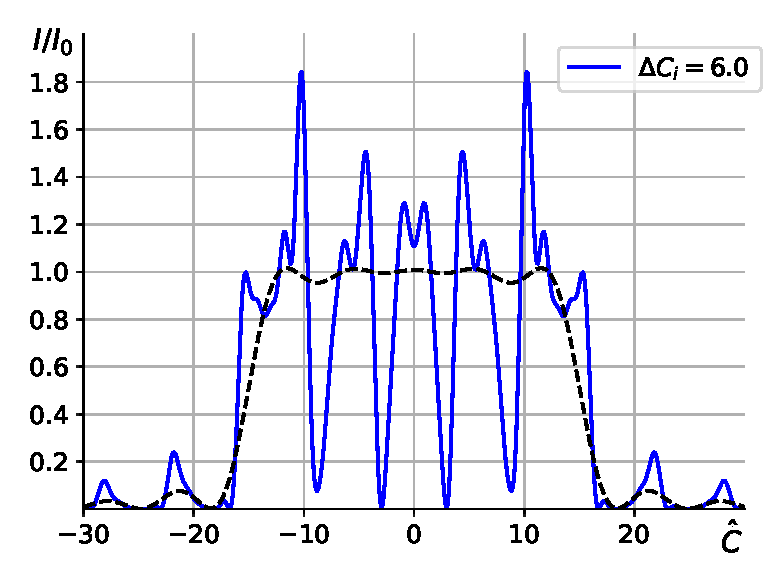
\includegraphics[width=\textwidth]{pic/spec_from_sec_und.pdf}
		\caption{}
		\label{fig:section_und_analitics}
	\end{minipage}\hfill
	\begin{minipage}{0.49\textwidth}
		\centering
		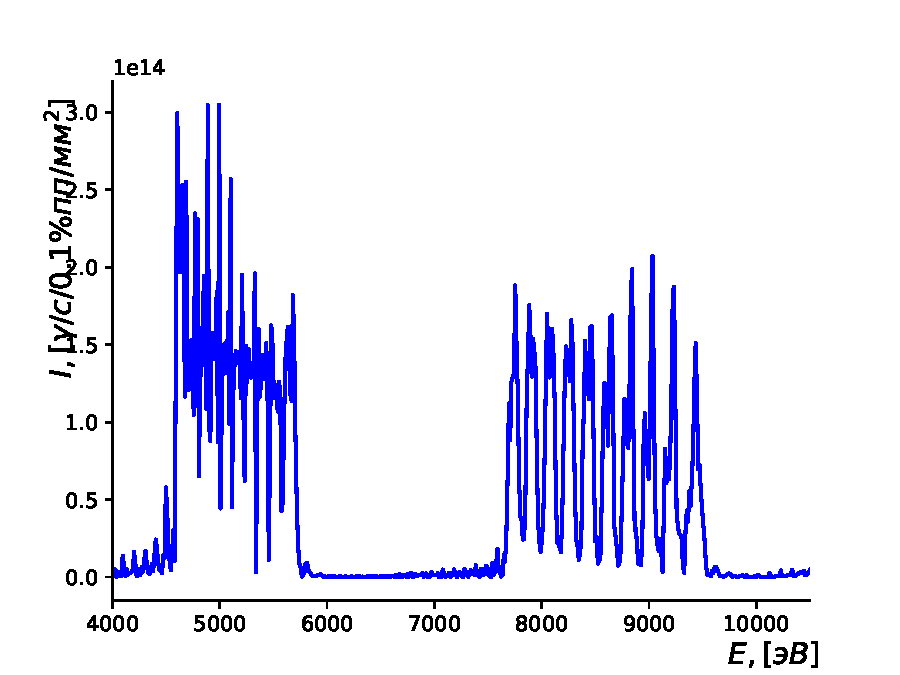
\includegraphics[width=\textwidth]{pic/spec_SRW.pdf}
		\caption{}
		\label{fig:section_und_SRW}
	\end{minipage}    
\end{figure}
На рис.~\ref{fig:section_und_SRW} показан характерный спектр секционного ондулятора посчитанного при помощи симуляционного кода SRW. Сравнение формы синей пунктирной линии на рис.~\ref{fig:section_und_analitics} и кривой на рис.~\ref{fig:section_und_SRW} показывает, что были сделаны правильные предположения в нашей аналитической модели, происходит интерференция между различными частями ондулятора.
Один из возможных путей, чтобы избавиться от интерференционных слагаемых в спектре ондуляторного излучения, добавить произвольную фазу между секциями ондулятора. Дело в том, что данные вычисления проводились для ондного электрона, если если мы хотим получить спектр, который получиться в точке наблюдения, то можно понять, что спектры на рис.~\ref{fig:section_und_analitics} синими линиями необходимо усреднить по числу электронов в пучке, усреднение по большому числу электронов даст спектр, который будет являть простой суммой $\sinc^2$ до каких либо дополнительных фаз, результат усреднения, приведёт к чёрной линии на рис.~\ref{fig:section_und_analitics}. Теперь здесь надо визуально показать процесс усреднения и заключить, что именно такой спектр будет наблюдаться на источнике.

\subsection{Учёт конечности эмиттанса}
В этом параграфе мы покажем влияние эмиттанса пучка на спектр излучения и угловое распределение. Для начала перепишем уравнение~\ref{eq:field_dist_Norm} с учётом отклонения частиц от заданной траектории, --- $h_x$ и $h_y$ и с некоторым дополнительным углом $\eta_x$ и $\eta_x$. Сразу можно понять, что в уравнениие~\ref{eq:field_dist_Norm} можно сделать замену $\theta_{x,y} \rightarrow \theta_{x,y} - \eta_{x, y} - \cfrac{l_{x,y}}{z_0}$ и переписать углы в нормализованных единицах аналогично с~\ref{eq:norm_units}, с точностью до фазы: 
\begin{equation}
	\label{eq:field_dist_Norm}
	\begin{array}{lcl}
	\hat{E}_{\bot} \sim
	\sinc\bigg[\cfrac{\hat{C}}{2} + 
	\cfrac{1}{4}\bigg(\hat{\theta}_{x} - \hat{\eta}_{x} - \cfrac{l_{x}}{z_0}\bigg)^2 +
	\cfrac{1}{4}\bigg(\hat{\theta}_{y} - \hat{\eta}_{y} - \cfrac{l_{y}}{z_0}\bigg)^2\bigg],
	\end{array}	
\end{equation}
При этом можно положить  $\cfrac{l_{x,y}}{z_0} \ll 1$, что выполняется с очень высокой точностью. 

В наших рассуждениях мы будем использовать один предельный случай: электронный пучок не симметричен его вертикальны размер много меньше размера по радиальному направлению. Распределение частиц будем считать гауссовым: 
\begin{equation}
	\label{eq:field_dist_Norm}
	h_{x, y}(\eta_{x, y}) = \cfrac{N_e}{\sqrt{2\pi}\sigma_{x', y'}} \exp[-\cfrac{\eta^2_{x, y}}{2\sigma^2_{x', y'}}]
\end{equation}

Для удобства перепишем это распределение в нормализованных единицах, помня $\sigma_{x', y'} = \epsilon_{x', y'}/\beta_{x', y'}$, где $\epsilon_{x', y'}$ --- вертикальный и горизонтальный эмиттансы, $\beta_{0x', y'}$ --- минимум бета-функции, обычно минимум бета-функции выбирают в середине ондулятора. Нормализованные единицы для $\hat{\beta}_{0} = \beta_{0}$
и $\hat{\epsilon} = (\omega/c)\epsilon$
\begin{equation}
	\label{eq:field_dist_Norm}
	h(\hat{\eta}) = \cfrac{1}{\sqrt{2\pi\hat{\epsilon}/\hat{\beta}}} \exp[-\cfrac{\hat{\eta}^2\hat{\beta}_{0}}{2\hat{\epsilon}^2}]
\end{equation}
Как уже упоминалось мы будем рассматривать предельный случай $\epsilon_{y'}/\beta_{y'} \ll 1$, в то время как $\hat{\beta_0}_{x,y} \sim 1$, поэтому просто $\epsilon_{y'} \ll 1$. Теперь можно записать интенсивность поля следующий образом: 
\begin{equation}
	\label{eq:convolution}
	\hat{I} = \cfrac{1}{\sqrt{2\pi\hat{\epsilon}/\hat{\beta}}}
	\displaystyle\int\limits_{-\infty}^{\infty} d\hat{\eta}_x \sinc^2(\zeta)	
	\exp[-\cfrac{\hat{\eta}_x^2\hat{\beta}_{0x}}{2\hat{\epsilon}_x}],д
\end{equation}
Где мы ввели $\zeta = \cfrac{\hat{C}}{2} + 
\cfrac{1}{4}(\hat{\theta}_{x} - \hat{\eta}_{x})^2 +
\cfrac{1}{4}\hat{\theta}_{y}^2$. Здесь мы учли, что распределение по $y$ действует как дельта-функция. Предыдущее уравнение упрощается дальше в пределе $\hat{\epsilon}_x\hat{\beta}_x \gg 1$, опять же помня, что и $\hat{\beta}_x \sim 1$, получается $\hat{\epsilon}_x \gg 1$. Ширина $\sinc^2(\zeta)$ много больше ширины гауссвоского распределения, ширина которого $\hat{\epsilon}_x$, поэтому интеграл будет набираться в пике кардинального синуса и экспоненту можно вынести с аргументом: $\hat{\eta}_x = \hat{\theta}_x$: 
\begin{equation}
	\label{eq:convolution}
	\hat{I} = \cfrac{\exp[-\hat{\theta}_x^2\hat{\beta}_{0x}/2\hat{\epsilon}_x]}{\sqrt{2\pi\hat{\epsilon}/\hat{\beta}}}
	\displaystyle\int\limits_{-\infty}^{\infty} d\hat{\eta}_x \sinc^2\bigg(\cfrac{\hat{C}}{2} + 
	\cfrac{1}{4}(\hat{\theta}_{x} - \hat{\eta}_{x})^2 +
	\cfrac{1}{4}\hat{\theta}_{y}^2\bigg)	
\end{equation}
Этот интеграл можно взять числено. %введя очевидную замену $\hat{\eta_{x}} \rightarrow \hat{\theta}_x - \hat{\eta_{x}}$. 
На~\ref{fig:2spec_emittance_and_single} представлены: линия 1.: спектр излучения пучка с $\hat{\epsilon}_x\rightarrow \infty$  $\hat{\epsilon}_x\rightarrow 0$, линия 2.: спектр одиночного электрона как функция $\hat{C} + \hat{\theta}_y^2/2$ при $\hat{\theta}_x = 0$, на рис.~\ref{fig:spec} тоже для распределения интенсивности по углам. 
\begin{figure}
	\centering  
	\begin{minipage}{0.49\textwidth}
		\centering
		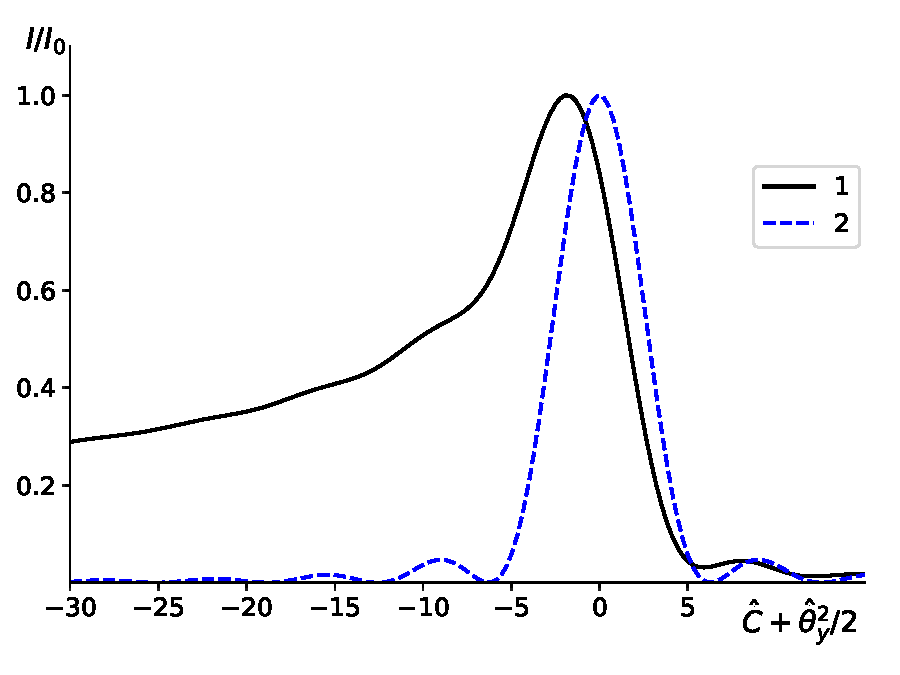
\includegraphics[width=\textwidth]{pic/spec_integ_emittance.pdf}
		\caption{}
		\label{fig:2spec_emittance_and_single}
	\end{minipage}\hfill
	\begin{minipage}{0.49\textwidth}
		\centering
		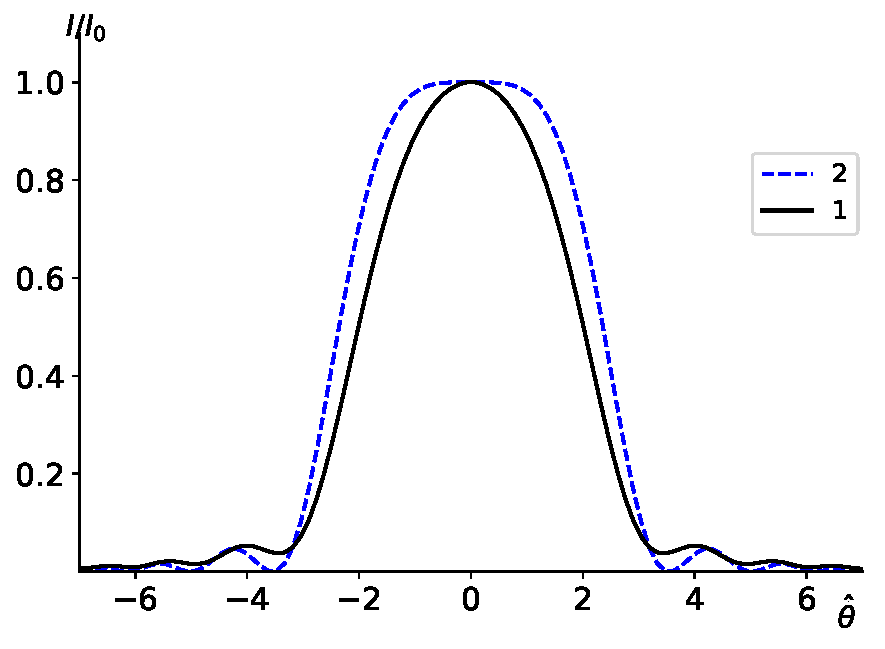
\includegraphics[width=\textwidth]{pic/angle_integ_emittance.pdf}
		\caption{}
		\label{fig:spec}
	\end{minipage}    
\end{figure}
\section{Фурье оптика}
В этой главе мы предложим наглядный подход к решению задачи о распространение волнового фронта в пустом пространстве, его прохождении через систему линзу. Приведённые результаты напрямую могут быть использованы в программном коде. Распределение поля в начальный момент времени будем считать гауссовским, однако, как будет видно из изложения, подход может быть использован для произвольного распределения поля. В наших выкладкам мы в полной мере следуем подходу (Салдин, Serkez), более детальное описание можно найти в (Гудман)

\subsection{Распространение света в пустом пространстве}
Наши рассуждения мы начнём с волнового уравнения в пустом пространстве ($\vec{j} = 0, \rho = 0$). 
\begin{equation}
	\pdv[2]{\vec{E}}{t} + c^2 \nabla^2 \vec{E} = 0
\end{equation}

В  $r\omega$-пространстве уравнение приобретает знакомый вид уравнения Гельмгольца, где $k_0 = \omega/c$.

\begin{equation}
	k_0^2\vec{\widetilde{E}} + \nabla^2 \vec{\widetilde{E}} = 0
\end{equation}

Совершив фурье-преобразование в $k$-пространство по координатам $x,y$, которое определим схожим образом с~\ref{eq:Fourier_wt}:

\begin{equation}
	\label{eq:Fourier_rk}
	\begin{array}{lcl}
		\vec{\widehat{E}}(\vec{k}, \omega) = \displaystyle\int\limits_{-\infty}^{\infty}\int\limits_{-\infty}^{\infty} dxdy \vec{E}(\vec{r}, t)\exp[ik_xx + ik_xx]\\
		\\
		\vec{E}(\vec{r}, \omega) = \cfrac{1}{4\pi^2}\displaystyle\int\limits_{-\infty}^{\infty}\int\limits_{-\infty}^{\infty} dk_xdk_y \vec{\widehat{E}}(\vec{k}, t)\exp[-ik_xx - ik_xx],
	\end{array}
\end{equation}

получим: 
\begin{equation}
	k_0^2\Big(1 - \cfrac{k^2_x}{k^2_0} - \cfrac{k^2_y}{k^2_0} \Big)\vec{\widehat{E}} + \dv[2]{\vec{\widehat{E}}}{z} = 0
\end{equation}

Теперь можно напрямую можно получить решение этого обыкновенного дифференциального уравнения:
\begin{equation}
	\vec{\widehat{E}}(\omega, k_x, k_y, z) = \vec{\widehat{E}}(\omega, k_x, k_y, 0)\exp[ik_0z\sqrt{1 - \frac{k^2_x}{k^2_0} - \frac{k^2_y}{k^2_0}} ]
\end{equation}

Введём функцию отклика среды:

\begin{equation}
	\begin{array}{lcl}
	H(k_x, k_y, z) = \cfrac{\vec{\widehat{E}}(\omega, k_x, k_y, z)}{\vec{\widehat{E}}(\omega, k_x, k_y, 0)} = \exp[ik_0z\sqrt{1 - \cfrac{k^2_x}{k^2_0} - \cfrac{k^2_y}{k^2_0}} ]
	\\
	\\
	H(k_x, k_y, z) \approxeq \exp[k_0z]\exp[-\cfrac{iz}{2k_0}(k^2_x + k^2_y)]
	\end{array}
\end{equation}
 
Видно, чтобы получить распределение электромагнитного поля на некотором расстоянии $z$, необходимо совершить обратное преобразование Фурье в $xy$-пространство. Таким образом решение волнового уравнения сводиться к трём относительно простым операциям: первое, --- перевод начального распределения в $k_xk_y$-пространство, далее домножение получившегося распределения на функцию отклика среды, в нашем случае пустое пространство, и последний шаг, --- обратное преобразование Фурье. 

\subsection{Действие тонкой линзы на волновой фронт}
В этом параграфе мы построим элементарную оптическую систему, состоящую из пустого промежутка, - $d_1$, тонкой линзы с оптической силой, - $1/f$ и ещё одного пустого промежутка до плоскости изображения. Действие тонкой линзы мы представим как прибавление к фазе волны следующего выражения: 
\begin{equation}
	T_f(x, y) = \exp[-\cfrac{ik_0}{2f}(x^2 + y^2)]
\end{equation}

Для предметности обсуждения определим Гауссов пучок: 

\begin{equation}
	\overline{E}(x, y, 0) = A\exp[-\cfrac{x^2 + y^2}{w^2_0}]
\end{equation}

После Фурье преобразования в $k_xk_y$-пространстве мы получим:

\begin{equation}
	\hat{E}(k_x, k_y, 0) = A\pi w^2_0\exp[-\cfrac{w^2_0}{4}(k_x^2 + k_y^2)]
\end{equation}

После домножения этого распределения поля в $k_xk_y$-пространстве на функцию отклика пустого промежутка, получим
\begin{equation}
	\label{eq:after_lens}
	\begin{array}{lcl}
	\hat{E}(k_x, k_y, z) = \hat{E}(k_x, k_y, z)H(k_x, k_y, z) 
	\\
	\\
	= A\pi w^2_0\exp[-\cfrac{w^2_0}{4}(k_x^2 + k_y^2)]\exp[k_0z]\exp[-\cfrac{iz}{2k_0}(k^2_x + k^2_y)]
	\\
	\\
	= A\pi w^2_0\exp[k_0z]\exp[-\cfrac{iq}{2k_0}(k^2_x + k^2_y)], 
	\end{array}
\end{equation}
здесь мы ввели $q = z - iz_R$, где $z_R = \cfrac{k_0w^2_0}{2}$. После перехода обратно в $xy$-пространство, получим: 
\begin{equation}
	\overline{E}(x, y, z) = \cfrac{iAk_0w^2_0}{2q}\exp[k_0z]\exp[-i\cfrac{k_0}{2q}(x^2 + y^2)],
\end{equation}
Теперь можно воспользоваться выражением для тонкой линзы и получить:
\begin{equation}
	\begin{array}{lcl}
	\overline{E}_{l}(x, y, z) = T_f(x, y)\overline{E}(x, y, z) = 
	\\
	\\
	\cfrac{iAk_0w^2_0}{2q}\exp[k_0z]\exp[-i\cfrac{k_0}{2q}(x^2 + y^2)]\exp[-\cfrac{ik_0}{2f}(x^2 + y^2)]
	\\
	\\
	\cfrac{iAk_0w^2_0}{2q}\exp[k_0z]\exp[-i\cfrac{k_0}{2q_l}(x^2 + y^2)],
	\end{array}
\end{equation}
где $\cfrac{1}{q_l} = \cfrac{1}{q} \; - \; \cfrac{1}{f}$. Теперь можно подвести итог: после распространения волнового фронта на расстояние $d_1$ параметр $q$ преобразуется:
\begin{equation}
	q(d_1) = q(0) + d_1, 
\end{equation}
далее на него действует линза: 
\begin{equation}
	\cfrac{1}{q_l} = \cfrac{1}{q(0) + d_1} - \cfrac{1}{f},
\end{equation}
и ещё один пустой промежуток, до места, где волновой фронт опять будет плоским: 
\begin{equation}
	q(d_1 + d_2) = q_l + d_2, 
\end{equation}
Условие того, что волновой фронт плоский мы сформулируем так, что $q(d_1 + d_2) = -i\cfrac{k_0w^2_2}{2}$, что легко проверятся подстановкой в~\ref{eq:after_lens}. Получим уравнение: 
\begin{equation}
	-i\cfrac{k_0w^2_2}{2} = q_l + d_2, 
\end{equation}
где, приравниванием мнимых частей получим: 
\begin{equation}
	w^2_2 = \cfrac{f^2w^2_1}{(f - d_1)^2 + (k_0w^2_1/2)^2}
\end{equation}
то же для реальных частей: 
\begin{equation}
	d_2 = f + f^2\cfrac{(d_1 - f)}{(d_1 - f)^2 + (k_0w^2_1/2)^2}
\end{equation}
Из последнего уравнения видно, что если положить перетяжку гауссового пучка раной нулю, то выражение переходит в обычное соотношение геометрической оптики.

В приведённой главе мы дали краткий путь того, как можно очень эффективно и относительно просто использовать Фурье оптику для написания симуляционных кодов при проектировании оптических систем. В качестве примера, для заинтересованных читателей на веб-странице (веб-страница) приведёт код простой оптической системы, который в полной мере используют результаты вышеприведённого параграфа. Код был написан автором данной рукописи рамках курса <<Основы вычислительной физики>>, который читается на физическом факультете НГУ. Дальнейшие комментарии к коду можно найти в репозитории указанной по ссылке.
\section{Краткий обзор дифракции на кристаллах}
В это главе мы кратко дадим основные результаты кинетической и динамической теории дифракции. Основные кристаллы используемы на синхротронных источниках третьего и четвёртого поколений - это $Si$ (кремний), $C$ (алмаз) и реже $Ge$ (германий), в виду свой кубической кристаллический решётки, эти кристаллы относительно просты для анализа. Для нас важны такие свойства кристаллов, как способность преобразовать относительно широкой спектр излучения ондулятора, в излучение с относительной монохроматичностью до $\Delta E/ E \sim 10^{-4}$, а также поглощательные способности кристаллов, что в значительной степени снижает тепловые нагрузки на оптические элементы.
\subsection{Симметричное брэгговское отражение от идеально кристалла}
Длины волн, которые отвечают резонансу при отражении падающего под углом $\theta$ к плоскости кристалла излучения, даётся законом Брэгга:  
%пропорциональный $\gamma / nN$, где $n$ --- номер гармоники излучения, $N$ --- число периодов ондулятора, а $\gamma$ --- гамма фактор релятивистского электрона
\begin{equation}
	m\lambda = 2d\sin\theta,
\end{equation}
где $d$ --- расстояние между плоскостями от которых происходит отражение, а $m$ --- некоторое положительно целое число. Основной результат, который мы будем использовать, это кривая Дарвина, которая определяет угловой акцептанс излучения. Динамическая и кинематическая теории дифракции дают конечную ширину в, которую кристалл может принять излучение, а также некоторый сдвиг, относительно предполагаемого брэгговского угла. На рис.~\ref{fig:bragg_R} показаны характерные кривые отражение. По ним видно, что чем больше энергия подающего пучка излучения, тем уже кривая и ближе к даваемому законом брэгга углу. При расчёте кристаллов монохроматоров этот факт необходимо учитывать, так как излучение не попавшее в акцептанс кристалла будет поглощаться и выделять в нем тепло. 
\subsection{Поглощательные способности кристаллов}
Одним из полезных применение кристаллов в рентгеновском диапазоне есть их фильтрующая способность, отрезать низкие энергии, в особенности для алмазных кристаллов, которые, по мимо всего, имеют хорошую теплопроводность, что способствуют быстрому теплоотводу. На рис.~\ref{fig:bragg_T} представлена кривая поглощения 100 мкм кристалла алмаза. Подобные кристаллы устанавливают перед первыми оптическими элементами, что в значительной степени снижает тепловые нагрузки, подавлением низших гармоник.
\begin{figure}
	\centering  
	\begin{minipage}{0.49\textwidth}
		\centering
		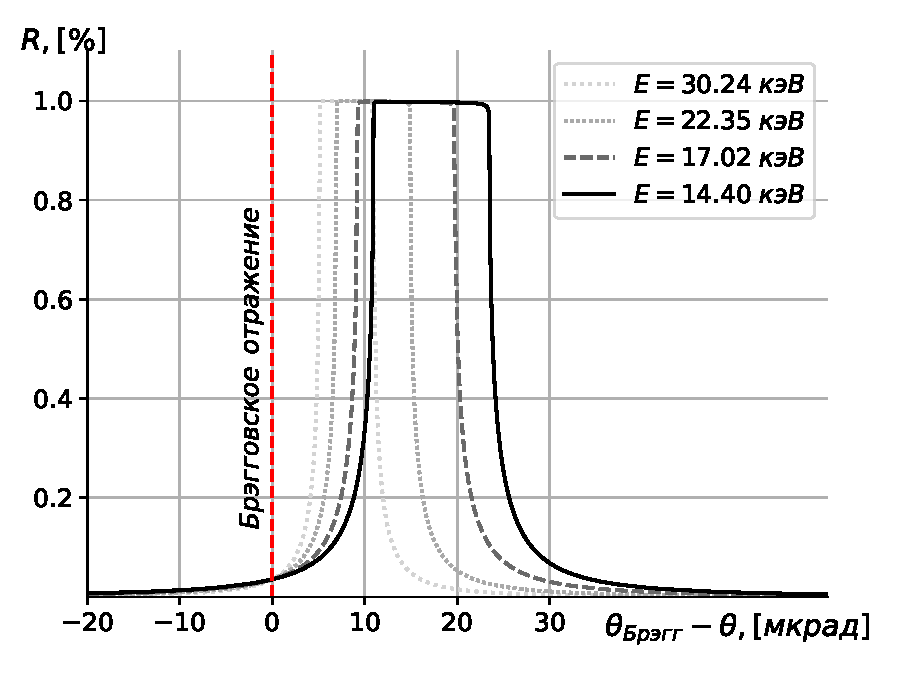
\includegraphics[width=\textwidth]{pic/bragg_R.pdf}
		\caption{}
		\label{fig:bragg_R}
	\end{minipage}\hfill
	\begin{minipage}{0.49\textwidth}
		\centering
		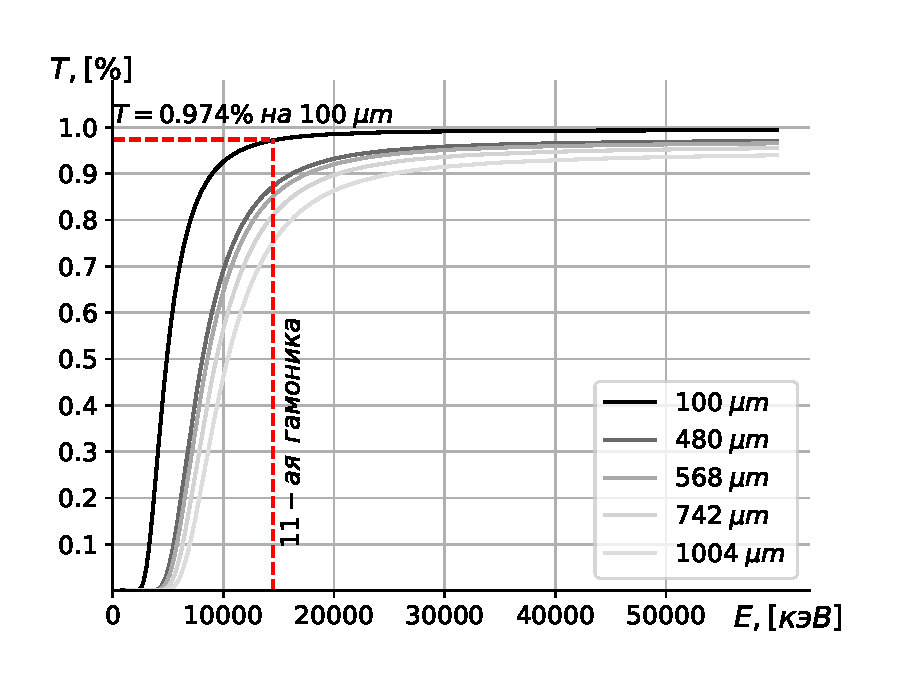
\includegraphics[width=\textwidth]{pic/bragg_T.pdf}
		\caption{}
		\label{fig:bragg_T}
	\end{minipage}    
\end{figure}























\chapter{Проектирование рентгенооптических трактов для Сибирского Кольцевого Источника Фонтов}

\section{Введение}
В данной главе мы рассмотрим схемы рентгенооптических трактов (здесь и далее, - бимлайнов), от источников высокого энергетических фотонов, - вставных устройств до деталей оптических компотен на билайне: фильтров, монохроматоров, рентгеновских зеркал. По большей части, будут обсуждаться станции первой очереди: 1-1 --- <<Микрофокус>>, 1-2 --- <<Структурная диагностика>>, 1-4 --- <<XAFS-спектроскопия и магнитный дихроизм>>.  
      % Заключение
%\clearpage                                  % В том числе гарантирует, что список литературы в оглавлении будет с правильным номером страницы
\phantomsection
\addcontentsline{toc}{chapter}{\bibname}	% Добавляем список литературы в оглавление
\hypersetup{ urlcolor=black }               % Ссылки делаем чёрными
%\providecommand*{\BibDash}{}                % В стилях ugost2008 отключаем использование тире как разделителя 
\urlstyle{rm}                               % ссылки URL обычным шрифтом
\insertbiblioother                          % Подключаем Bib-базы
\urlstyle{tt}                               % возвращаем установки шрифта ссылок URL
%\hypersetup{ urlcolor={urlcolor} }          % Восстанавливаем цвет ссылок      % Список литературы
\clearpage
\phantomsection
\addcontentsline{toc}{chapter}{\listfigurename}
\listoffigures									% Список изображений


%%% Список таблиц %%%
% (ГОСТ Р 7.0.11-2011, 5.3.10)
\clearpage
\phantomsection
\addcontentsline{toc}{chapter}{\listtablename}
\listoftables									% Список таблиц
\newpage           % Списки таблиц и изображений (иллюстративный материал)

%\appendix
%% Правка оформления ссылок на приложения:
%http://tex.stackexchange.com/questions/56839/chaptername-is-used-even-for-appendix-chapters-in-toc
%http://tex.stackexchange.com/questions/59349/table-of-contents-with-chapter-and-appendix
%% требует двойной компиляции
\addtocontents{toc}{\def\protect\cftchappresnum{\appendixname{} }%
\setlength{\cftchapnumwidth}{\widthof{\cftchapfont\appendixname~Ш\cftchapaftersnum}}%
}
%% Оформление заголовков приложений ближе к ГОСТ:
\sectionformat{\chapter}[display]{% Параметры заголовков разделов в тексте
    label=\chaptertitlename\ \thechapter,% (ГОСТ Р 2.105, 4.3.6)
    labelsep=20pt,
}
\renewcommand\thechapter{\Asbuk{chapter}} % Чтобы приложения русскими буквами нумеровались
\chapter{Единицы измерения потока фотонов}
В области синхротронного излучения приняты специфические единицы измерения потока фотонов:
\begin{equation}
	\Phi = \cfrac{\gamma}{\textup{сек} \cdot 0.1\%\textup{bw} \cdot \textup{мм}^2}
\end{equation}
Для удобства пользователей этого излучения, была введено необычное единица $0.1\%\textup{bw}$, что можно интерпретировать следующим образом, --- это количество фотонов попавшее в полосу пропускания шириной $0.1\%$ на некоторой фиксированной энергии гамма-квантов, т.е., например, для энергии $1000 \textup{eV}$ ширина полосы будет в диапазоне $999,5 - 1000,5 \textup{eV}$. Данная единица была введена, для удобства оценок потоков, после прохождения излучения через кристаллические монохроматоры и решёточные монохроматоры, полосы пропускания которых как раз составляют порядка $10^{-3} - 10^{-4}$. 

Иногда возникает потребность, для удобства, перевести эти единицы, например, к следующему виду:
\begin{equation}
\Phi = \cfrac{\gamma}{\textup{сек} \cdot \textup{eV} \cdot \textup{мм}^2}
\end{equation} 
Сделать это можно следующим образом, необходимо поточено умножить спектральное распределение на множитель $\cfrac{0.1 \% \cdot E_{ph}}{1\textup{eV}}$, что даст необходимые единицы измерения. Далее, спектр можно привести к:
\begin{equation}
\Phi = \cfrac{W}{\textup{eV} \cdot \textup{мм}^2},
\end{equation} 
Так спектральное распределение легко интегрировать, чтобы получить, например, полную плотность мощности излучения и делать оценки тепловых нагрузок на оптические элементы.
\chapter{Краткий обзор дифракции на кристаллах}
В этой главе мы кратко дадим основные результаты кинетической и динамической теории дифракции. Основные кристаллы используемы на источниках синхротронного излучения --- это $Si$ (кремний), $C$ (алмаз) и реже $Ge$ (германий). Виду кубической кристаллической решётки эти кристаллы относительно просты при рассмотрение динамики отражение и преломления на кристаллических плоскостях. Для нас важны такие свойства кристаллов, как способность преобразовать относительно широкой спектр ондуляторного излучения в излучение с относительной монохроматичностью до $\Delta E/ E \sim 10^{-4}$. Также мы дадим основную информация по поглощательным способностям кристаллов
\section{Симметричное брэгговское отражение от идеально кристалла}
Длины волн, которые отвечают резонансу при отражении падающего под углом $\theta$ к плоскости кристалла излучения, даётся законом Брэгга:  
%пропорциональный $\gamma / nN$, где $n$ --- номер гармоники излучения, $N$ --- число периодов ондулятора, а $\gamma$ --- гамма фактор релятивистского электрона
\begin{equation}
	m\lambda = 2d\sin\theta,
\end{equation}
где $d$ --- расстояние между плоскостями от которых происходит отражение, $m$ --- некоторое положительно целое число. Однако динамическая и кинематическая теории дифракции уточнаю данные результат и вносят конечную угловую и/или по энергии ширину, в которую кристалл может принять излучение, а также некоторый сдвиг, относительно предполагаемого брэгговского угла.  Кривая, которая описывает отражательную способность кристалла, называется кривой Дарвина, именно она определяет угловой и/или энергетический акцептанс излучения. На рис.~\ref{fig:bragg_R} показаны характерные кривые отражение для алмаза и кремния. 
\begin{figure}
	\centering  
	\begin{minipage}{0.49\textwidth}
		\centering
		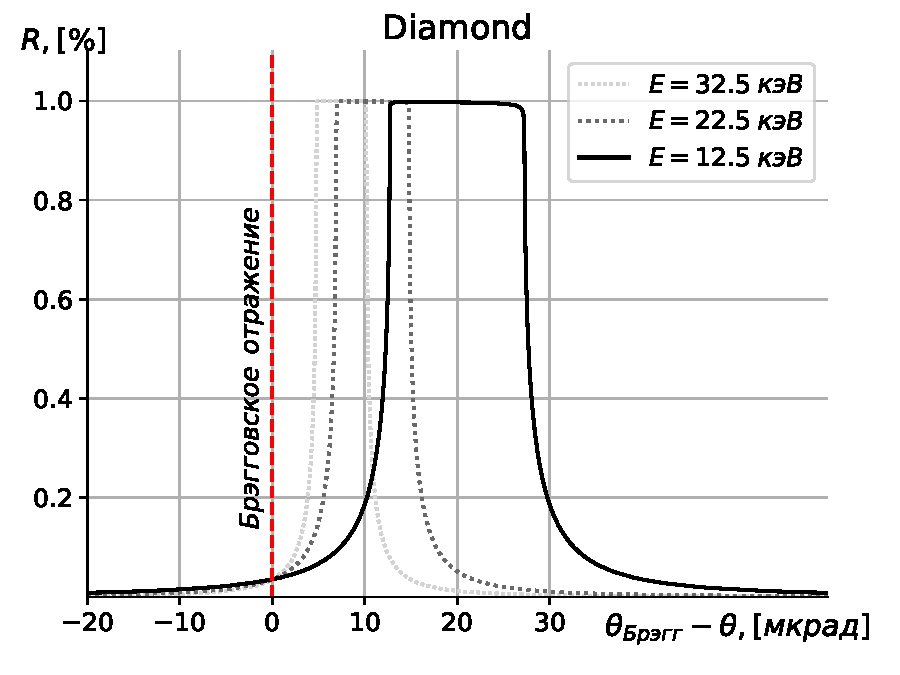
\includegraphics[width=\textwidth]{pic/Diamond_bragg_R.pdf}
		\caption{Кривая брегга для алмаза на разных энергиях}
		\label{fig:bragg_R}
	\end{minipage}\hfill
	\begin{minipage}{0.49\textwidth}
		\centering
		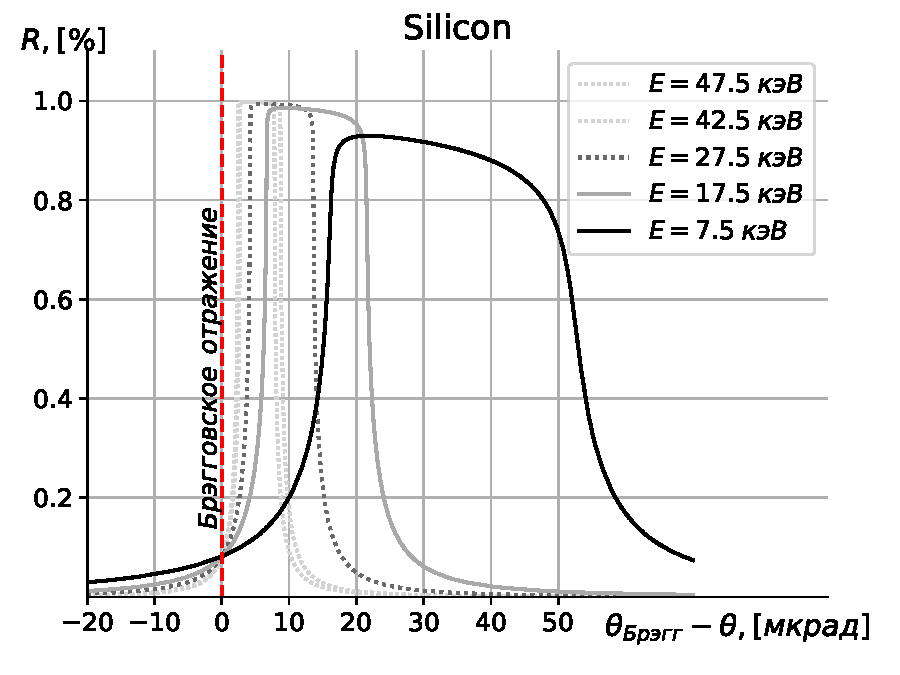
\includegraphics[width=\textwidth]{pic/Silicon_bragg_R.pdf}
		\caption{Кривая брегга для кремния на разных энергиях}
		\label{fig:bragg_T}
	\end{minipage}    
\end{figure}
По ним видно, чем больше энергия подающего пучка излучения, тем  кривая уже и ближе к даваемому законом брэгга углу. При расчёте кристаллов монохроматоров этот факт необходимо учитывать, для эффективной работы кристалла и уменьшения тепловых нагрузок, угловая расходимость кристалла должна входить в акцептанс кристалла, иначе излучение поглотится в кристалле, что крайне нежелательно. Кривые ассиметричны по правому краю, теория дифракции объясняет данный факт большим поглощением на низких энергиях.

В целом, данной информации достаточно, чтобы иметь первое представление о разработке оптических трактов синхротронного излучения. Для дальнейшего чтения и углубления знаний в данном вопросе могут быть полезны следующие книги \cite{als2011elements}, \cite{authier2006dynamical}.

\section{Поглощательные способности кристаллов}
Одним из полезных применений кристаллов в рентгеновском диапазоне есть их фильтрующая способность, отрезать низкие энергии, в особенности для алмазных кристаллов, которые, по мимо всего, имеют хорошую теплопроводность, что способствуют быстрому теплоотводу. На рис.~\ref{fig:bragg_T} представлена кривая поглощения 100 мкм кристалла алмаза. Подобные кристаллы устанавливают перед первыми оптическими элементами, что в значительной степени снижает тепловые нагрузки, подавляя низшие гармоники, в нашем случае ондуляторного излучения. 
\chapter{Дополнительные графики} \label{AppendixA}

\chapter{Примеры программного кода} \label{AppendixB}

\section{Подраздел приложения}\label{AppendixB1}

\normalsize% возвращаем шрифт к нормальному
        % Приложения

\end{document}
